%\documentclass[12pt,a4paper]{report}
%\usepackage[utf8]{inputenc}
%\usepackage{amsmath}
%\usepackage{amsfonts}
%\usepackage{amssymb}
%\usepackage[margin=2.5cm]{geometry}
%\usepackage{graphicx}
%\usepackage{caption}
%\usepackage{subcaption}
%\usepackage[nottoc,numbib]{tocbibind}
%\linespread{1.3}
%\begin{document}
\chapter{Introduction}
\label{Introduction}
	Graphene is an allotope of carbon in the form of a single atomic layer of graphite. The term graphene was first used in 1962 \cite{b68} and is considered to be the first in a new range of two dimensional materials. The occurence of two dimensional materials in nature was originally unknown due to thermal fluctuations which may destroy the structure \cite{b64, b69}, until thin carbon films (including graphene) were extracted from graphite via mechanical exfoliation \cite{b65, b70}. The discrepancy between theoretical predictions and the discovery of graphene was later resolved as the two dimensional materials would experience microscopic corrugations in the third dimension \cite{b66, b67}. These corrugations, or ripples on the nanometre scale allow suspended graphene to be stable in three dimensional space despite the thermodynamic instabilities which do not allow two dimensional materials to exist in nature.

	The structure of graphene is a two dimensional hexagonal lattice \cite{b5} and will be discussed mathematically in the following section. The interesting properties of graphene arise due to the way the carbon atoms are bonded. The carbon atom contains 6 protons and therefore 6 electrons. Two of these electrons are located in the 1s$^2$ orbital, which is too close to the nucleus to contribute to bonding. The remaining electrons are found in the 2s$^2$ and 2p$^2$ orbitals which are free to form covalent bonds. As only 3 conventional covalent bonds are formed in a hexagonal lattice, the spare electron causes $sp^{2}$ hybridisation which results in an out of plane $\pi$ bond \cite{b46, b62}. The structure of graphene is responsible for its impressive physical properties such as a Young's modulus of 1 TPa \cite{b58, b63}, intrinsic strength of 130 Gpa \cite{b58}, thermal conductivity of 2000–4000 W m$^{-1}$ K$^{-1}$ \cite{b60} and an intrinsic mobility of 2 x 10$^{5}$ cm$^{2}$ V$^{-1}$ s$^{-1}$ \cite{b45, b61}. 
%%%%%
%%%%%
%%%%%
	\section{Structure}
	\label{Introduction - Structure}
		This section explains the structure of graphene. The hexagonal structure of graphene can be constructed with two triangular lattices. Atoms in each of these lattices will be refered to as A or B depending on which triangular lattice they reside on. There are two orientations which are often used which are essentially a rotation, however depending on the situation one may be more convenient.
%%%%%
%%%%%
%%%%%
		\subsection{Zig-Zag Orientation}
		\label{Introduction - Zig-Zag Orientation}
			The first step to deriving the structure of the lattice is to define the inter-atomic distance $a=0.142$ nm \cite{b8}. This quantitiy can then be used to find vectors that describe the locations of the next nearest atom. For zig-zag orientation the nearest neighbor vectors can be found to be \cite{b1}:
			\begin{figure}[h]
				 \begin{subfigure}[h]{0.47\textwidth}
					\centerline{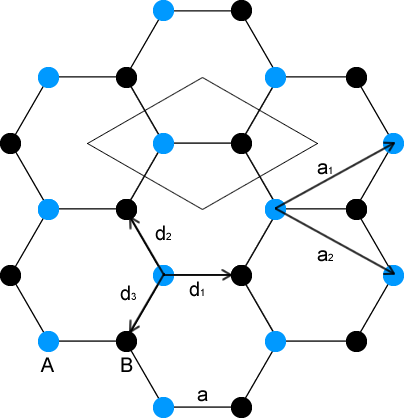
\includegraphics[scale=0.5]{images/strucure-zig-flat}}
					\caption{}
				\end{subfigure}
				\hspace{1cm}
				\begin{subfigure}[h]{0.47\textwidth}
					\centerline{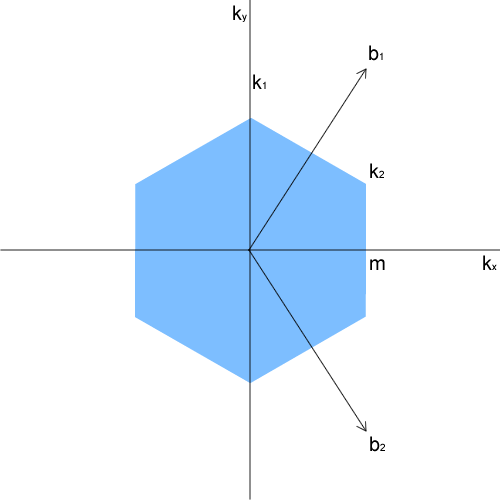
\includegraphics[scale=0.42]{images/strucure-bz-zig-flat}}
					\caption{}
				\end{subfigure}
				\caption{(a) The lattice vectors $\vec{a}_{1},\vec{a}_{2}$, nearest neighbor vectors $\vec{d}_{1},\vec{d}_{2},\vec{d}_{3}$, unit cell,  the carbon-carbon bond length $a=0.142$ nm and the sub lattices A and B. (b) The Brillouin zone with reciprocal lattice vectors $\vec{b}_{1},\vec{b}_{2}$, Dirac points $k_{1},k_{2}$ and point $m$.}
				\label{introduction-structure-zig}
			\end{figure}
			\begin{align}
				\vec{d}_{1}=a\left(1,0\right)\hspace{1cm}\vec{d}_{2}=\frac{a}{2}\left(-1,\sqrt{3}\right)\hspace{1cm}\vec{d}_{3}=\frac{a}{2}\left(-1,-\sqrt{3}\right)
			\end{align}
			Using the nearest neighbor vectors the lattice vectors can be found. These lattice vectors are for the individual triangular lattices and show the locations of the other atoms on the same lattice. To show the full hexagonal lattice these lattice vectors should start from an A and a B atom. The lattice vectors in zig-zag orientation are \cite{b1}:
			\begin{align}
				\vec{a}_{1}=\vec{d}_{1}-\vec{d}_{3}=\frac{a}{2}\left(3,\sqrt{3}\right)\hspace{1cm}\vec{a}_{2}=\frac{a}{2}\left(3,-\sqrt{3}\right)
			\end{align}
			The reciprocal lattice vectors are defined as:
			\begin{align}
				\vec{b}_{1}=2\pi\frac{\vec{a}_{2}\times\vec{a}_{z}}{\vec{a}_{1}\cdot\vec{a}_{2}\times\vec{a}_{z}}\hspace{1cm}\vec{b}_{2}=2\pi\frac{\vec{a}_{z}\times\vec{a}_{1}}{\vec{a}_{1}\cdot\vec{a}_{2}\times\vec{a}_{z}}
			\end{align}
			As graphene is two dimensional, the z components of $\vec{a}_{1}$ and $\vec{a}_{2}$ can be taken to be zero with $\vec{a}_{z}$ as the z direction unit vector. With the definitions of $\vec{a}_{1}$ and $\vec{a}_{2}$ the reciprocal lattice vectors become \cite{b1}:
			\begin{align}
				\vec{b_{1}}=\frac{2\pi}{3a}\left(1,\sqrt{3}\right)\hspace{1cm}\vec{b_{2}}=\frac{2\pi}{3a}\left(1,-\sqrt{3}\right)
			\end{align}
			In later sections the points where the valance and conduction bands meet will be studied, these are known as Dirac points. The locations of the Dirac points $k_{1}, k_{2}$ are at the corners of the Brillouin zone. Due to the symmetry of graphene only two Dirac points need to be found. Using the reciprocal lattice vectors and the half way point $m$:
			\begin{align}
				|m|=\frac{|\vec{b_{1}}|}{2}\hspace{1cm}|\vec{b_{1}}|=\sqrt{\left(\frac{2\pi}{3a}\right)^{2}+\left(\frac{2\pi\sqrt{3}}{3a}\right)^{2}}=\frac{4\pi}{3a}
			\end{align}
			the Dirac points can be found.
			\begin{align}
				k_{1}&=\left(0,\sqrt{\left(\frac{2\pi}{3a}\right)^{2}+\left(\frac{2\pi}{3a\sqrt{3}}\right)^{2}}\right)=\left(0,\frac{4\pi}{3\sqrt{3}a}\right)\\
				k_{2}&=\left(|m|,\frac{|m|}{\sin(\pi/3)}\sin(\pi/6)\right)=\left(\frac{2\pi}{3a},\frac{2\pi}{3a\sqrt{3}}\right)
			\end{align}
			The unit cell and all previously derived vectors for graphene have been included in Figure \ref{introduction-structure-zig}.
%%%%%
%%%%%
%%%%%
		\subsection{Armchair Orientation}
		\label{Introduction - Armchair Orientation}
			The same calculations can then be made to find the vectors for armchair orientation, this is a rotation of $30^{\circ}$, which can be useful as the $y$ component of $\vec{a}_{4}$ becomes zero.
			\begin{figure}[h]
				 \begin{subfigure}[h]{0.47\textwidth}
					\centerline{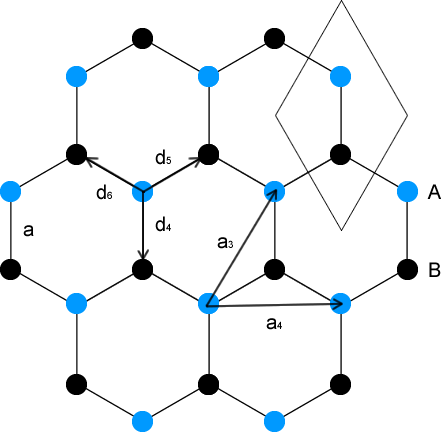
\includegraphics[scale=0.5]{images/strucure-arm-flat}}
					\caption{}
				\end{subfigure}
				\hspace{1cm}
				\begin{subfigure}[h]{0.47\textwidth}
					\centerline{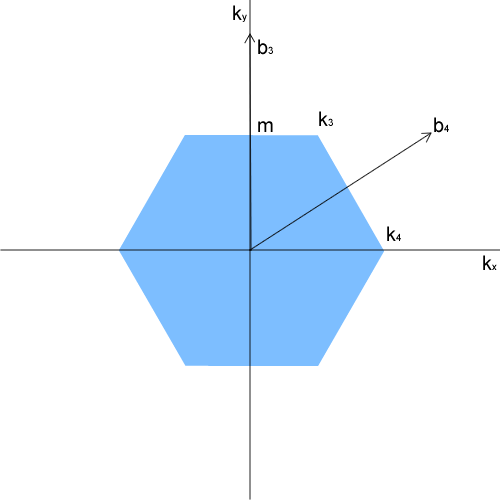
\includegraphics[scale=0.43]{images/strucure-bz-arm-flat}}
					\caption{}
				\end{subfigure}
				\caption{(a) The lattice vectors $\vec{a}_{3},\vec{a}_{4}$, nearest neighbor vectors $\vec{d}_{4},\vec{d}_{5},\vec{d}_{6}$, unit cell, the carbon-carbon bond length $a=0.142$ nm and the sub lattices A and B. (b) The Brillouin zone with reciprocal lattice vectors $\vec{b}_{3},\vec{b}_{4}$, Dirac points $k_{3},k_{4}$ and the mid point $m$.}
				\label{introduction-structure-armchair}
			\end{figure}
			The nearest neighbor vectors in this rotation are then \cite{b55}:
			\begin{align}
				\vec{d}_{4}=a\left(0,-1\right)
				\hspace{1cm}
				\vec{d}_{5}=\frac{a}{2}\left(\sqrt{3},1\right)
				\hspace{1cm}
				\vec{d}_{6}=\frac{1}{2}\left(-\sqrt{3},1\right)
			\end{align}
			with lattice vectors:
			\begin{align}
				\vec{a}_{3}=\frac{a}{2}\left(\sqrt{3},3\right)\hspace{1cm}\vec{a}_{4}=a\sqrt{3}\left(1,0\right)
			\end{align}
			reciprocal lattice vectors:
			\begin{align}
				\vec{b}_{3}=\frac{4\pi}{3a}\left(0,1\right)\hspace{1cm}\vec{b}_{4}=\frac{2\pi}{3a}\left(\sqrt{3},1\right)
			\end{align}
			and Dirac points:
			\begin{align}
				k_{3}=\frac{2\pi}{3a}\left(\frac{1}{\sqrt{3}},1\right)\hspace{1cm}k_{4}=\frac{4\pi}{3\sqrt{3}a}\left(1,0\right)
			\end{align}
			The unit cell and all other vectors for armchair graphene are shown in Figure \ref{introduction-structure-armchair}.
%%%%%
%%%%%
%%%%%
\section{Tight Binding Approximation}
\label{Introduction - Tight Binding Approximation}
	The tight binding approximation will reveal the full energy spectrum for the graphene hexagonal lattice. This is done by asigning each electron a Bloch wave-function and allowing it to hop to other atoms in the lattice. Other atoms are located using the lattice and neighbor vectors from Section \ref{Introduction - Structure}. In this section vectors for the zig-zag orientation will be used as shown in Figure \ref{introduction-tb-diagram} and derived in Section \ref{Introduction - Zig-Zag Orientation}. Depending on the range of hopping allowed; the accuracy of this approximation will increase.
	\begin{figure}[h]
		\begin{align}
			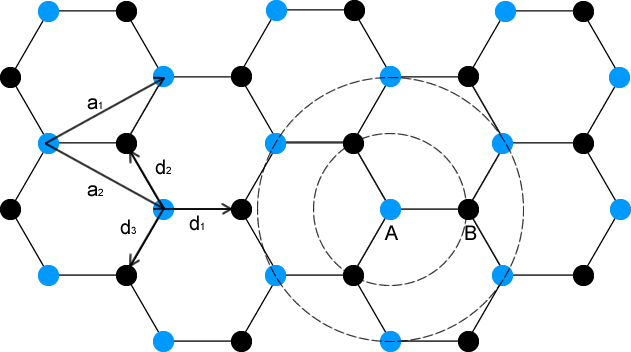
\includegraphics[scale=0.5]{images/tight-binding-flat}		
		\end{align}
		\caption{The graphene structure used for the tight binding approximation. The nearest neighbor vectors $\vec{d}_{1,2,3}$ and lattice vectors $\vec{a}_{1,2}$ have been included as defined in Section \ref{Introduction - Zig-Zag Orientation}. The radius for nearest neighbor and second nearest neighbor hopping is shown centered at an A site atom.}
		\label{introduction-tb-diagram}
	\end{figure}
%%%%%
%%%%%
%%%%%
	\subsection{Nearest Neighbor Only}
		\label{nearest-neighbor-only}
		Here only nearest neighbor hopping will be considered. This condition only allows hopping from A sites to B sites and vice versa. The Bloch wave-function \cite{b44} is defined as:
		\begin{equation}							 \psi_{k}\left(\vec{r}\right)=\sum\limits_{\vec{R}}e^{i\vec{k}\cdot\vec{R}}\left(b_{a}\varphi_{a}\left(\vec{r}+\vec{R}\right)+b_{b}\varphi_{b}\left(\vec{r}+\vec{R}\right)\right)
		\end{equation}
		Due to the symmetry of the graphene lattice all the wave-functions will be equivalent, however the interaction from a B site electron to an A site atom will be shifted by some vector $\vec{d}$, thus for an A site atom the wave-functions for an electron on the A lattice and B lattice can be defined as:
		\begin{align}
 			\varphi_{a}\left(\vec{r}\right)\equiv\varphi\left(\vec{r}\right)\hspace{1cm}\varphi_{b}\left(\vec{r}\right)\equiv\varphi\left(\vec{r}+\vec{d}_{1}\right)
		\end{align}
		The opposite will be true for a B site atom. For a B site atom the wave-functions for electrons from each lattice are defined as:
		\begin{align}
 			\varphi_{b}\left(\vec{r}\right)\equiv\varphi\left(\vec{r}\right)\hspace{1cm}\varphi_{a}\left(\vec{r}\right)\equiv\varphi\left(\vec{r}-\vec{d}_{1}\right)
		\end{align}
			The Schr{\" o}dinger equation can take the form:
			\begin{align}
				\langle\varphi_{a,b}|\hat{H}|\psi_{k}\rangle&=\varepsilon_{k}\langle\varphi_{a,b}|\psi_{k}\rangle\\
				\langle\varphi_{a,b}|(\hat{H}_{\mathrm{atomic}}+\Delta u)|\psi_{k}\rangle&=E\langle\varphi_{a,b}|\psi_{k}\rangle+\langle\varphi_{a,b}|\Delta u|\psi_{k}\rangle
			\end{align}
			Here the Schr{\" o}dinger equation has been split into the atomic component and an external potential; $\varepsilon_{k}$ is the energy of the whole system, $E$ is the energy of the atomic $p_{z}$ orbital electron and $\Delta u$ is an external potential. With this definition of the Schr{\" o}dinger equation and the previous definitions for electrons at A and B sites, the bra-kets can be evaluated, so for an A site:
			\begin{align}
				\langle\varphi_{a}|\psi_{k}\rangle=\sum\limits_{\vec{R}}e^{i\vec{k}\cdot\vec{R}}\left(b_{a}\int\varphi^{*}\left(\vec{r}\right)\varphi\left(\vec{r}+\vec{R}\right)d\vec{r}+b_{b}\int\varphi^{*}\left(\vec{r}\right)\varphi\left(\vec{r}+\vec{R}+\vec{d}_{1}\right)d\vec{r}\right)
				\label{introduction-start-tb}
			\end{align}
			Then for nearest neighbor atoms the vector $\vec{R}$ can only be:
			\begin{align}
				\vec{R}=0, -\vec{a}_{1}, -\vec{a}_{2}
			\end{align}
			Similarly for a B site:
			\begin{align}
				\langle\varphi_{b}|\psi_{k}\rangle=\sum\limits_{\vec{R}}e^{i\vec{k}\cdot\vec{R}}\left(b_{a}\int\varphi^{*}\left(\vec{r}\right)\varphi\left(\vec{r}+\vec{R}-\vec{d}_{1}\right)d\vec{r}+b_{b}\int\varphi^{*}\left(\vec{r}\right)\varphi\left(\vec{r}+\vec{R}\right)d\vec{r}\right)
				\label{introduction-start-tb-b}
			\end{align}
			and the vector $\vec{R}$:
			\begin{align}
				\vec{R}=0, \vec{a}_{1}, \vec{a}_{2}
			\end{align}
			Evaluating the sums and removing any terms which didn't reach atoms:
			\begin{align}
				\langle\varphi_{a}|\psi_{k}\rangle&=b_{a}\int\varphi^{*}\left(\vec{r}\right)\varphi\left(\vec{r}\right)d\vec{r}+b_{b}\int\varphi^{*}\left(\vec{r}\right)\varphi\left(\vec{r}+\vec{d}_{1}\right)d\vec{r}\\
				&+e^{-i\vec{k}\cdot\vec{a}_{1}}b_{b}\int\varphi^{*}\left(\vec{r}\right)\varphi\left(\vec{r}+\vec{d}_{3}\right)d\vec{r}+e^{-i\vec{k}\cdot\vec{a}_{2}}b_{b}\int\varphi^{*}\left(\vec{r}\right)\varphi\left(\vec{r}+\vec{d}_{2}\right)d\vec{r}\\
				\langle\varphi_{b}|\psi_{k}\rangle&=b_{a}\int\varphi^{*}\left(\vec{r}\right)\varphi\left(\vec{r}-\vec{d}_{1}\right)d\vec{r}+b_{b}\int\varphi^{*}\left(\vec{r}\right)\varphi\left(\vec{r}\right)d\vec{r}\\
				&+e^{i\vec{k}\cdot\vec{a}_{1}}b_{a}\int\varphi^{*}\left(\vec{r}\right)\varphi\left(\vec{r}-\vec{d}_{3}\right)d\vec{r}+e^{i\vec{k}\cdot\vec{a}_{2}}b_{a}\int\varphi^{*}\left(\vec{r}\right)\varphi\left(\vec{r}-\vec{d}_{2}\right)d\vec{r}
			\end{align}
			As the graphene sheet is symmetrical, the probability of an electron hopping from an A site to a B site will be the same as an electron hopping from a B site to an A site, this probability will be defined as:
			\begin{align}
				\int\varphi^{*}\left(\vec{r}\right)\varphi\left(\vec{r}-\vec{d}_{1,2,3}\right)d\vec{r}=\int\varphi^{*}\left(\vec{r}\right)\varphi\left(\vec{r}+\vec{d}_{1,2,3}\right)d\vec{r}\equiv\alpha
			\end{align}
			As $\int\varphi^{*}\left(\vec{r}\right)\varphi\left(\vec{r}\right)d\vec{r}$ must be equal to one from normalisation the bra-kets for A and B sites become:
			\begin{align}
				\langle\varphi_{a}|\psi_{k}\rangle&=b_{a}+b_{b}\alpha\left(1+e^{-i\vec{k}\cdot\vec{a}_{1}}+e^{-i\vec{k}\cdot\vec{a}_{2}}\right)\\
				\langle\varphi_{b}|\psi_{k}\rangle&=b_{b}+b_{a}\alpha\left(1+e^{i\vec{k}\cdot\vec{a}_{1}}+e^{i\vec{k}\cdot\vec{a}_{2}}\right)
			\end{align}
			The same method can be applied to $\langle\varphi_{a,b}|\Delta u|\psi_{k}\rangle$  with the definitions:
			\begin{align}
				\beta\equiv\int\varphi^{*}\left(\vec{r}\right)\Delta u\left(\vec{r}\right)\varphi\left(\vec{r}\right) d\vec{r}\hspace{1cm}t\equiv\int\varphi^{*}\left(\vec{r}\right)\Delta u\left(\vec{r}\right)\varphi\left(\vec{r}+\vec{d}_{1,2,3}\right) d\vec{r}
			\end{align}
			Which results in:
			\begin{align}
				\langle\varphi_{a}|\Delta u|\psi_{k}\rangle&=b_{a}\beta+b_{b}t\left(1+e^{-i\vec{k}\cdot\vec{a}_{1}}+e^{-i\vec{k}\cdot\vec{a}_{2}}\right)\\
				\langle\varphi_{b}|\Delta u|\psi_{k}\rangle&=b_{b}\beta+b_{a}t\left(1+e^{i\vec{k}\cdot\vec{a}_{1}}+e^{i\vec{k}\cdot\vec{a}_{2}}\right)
			\end{align}
			The previously derived values of $\vec{a}_{1}, \vec{a}_{2}$ can be used to define $f\left(\vec{k}\right)$ as:
			\begin{equation}
				f\left(\vec{k}\right)\equiv 1+e^{-i\vec{k}\cdot\vec{a}_{1}}+e^{-i\vec{k}\cdot\vec{a}_{2}}=1+2e^{-i\left(\frac{3ak_{x}}{2}\right)}\cos\left(\frac{\sqrt{3}ak_{y}}{2}\right)
				\label{introduction-fk}
			\end{equation}
			With the bra-kets evaluated the total energy of the system $\varepsilon_{k}\langle\varphi_{a,b}|\psi_{k}\rangle=E\langle\varphi_{a,b}|\psi_{k}\rangle+\langle\varphi_{a,b}|\Delta u|\psi_{k}\rangle$ can be written as:
			\begin{align}
				b_{a}\left(\varepsilon_{k}-E+\beta\right)+b_{b}f\left(\vec{k}\right)\left(\left(\varepsilon_{k}-E\right)\alpha+t\right)&=0\\
				b_{b}\left(\varepsilon_{k}-E+\beta\right)+b_{a}f^{*}\left(\vec{k}\right)\left(\left(\varepsilon_{k}-E\right)\alpha+t\right)&=0
			\end{align}
			Since $\Delta u\left(\vec{r}\right)$ will be large at $\vec{r}+\vec{d}_{1}$, it can be assumed that $\varphi\left(\vec{r}+\vec{d}_{1}\right)\ll\Delta u\left(\vec{r}\right)\varphi\left(\vec{r}+\vec{d}_{1}\right)$ and therefore $\alpha\ll t$ and $\alpha=0$. These simultaneous equations can then be written in matrix from:
			\begin{align}
				\left[\begin{array}{ccc}
					\varepsilon_{k}-E+\beta&t f\left(\vec{k}\right)\\
					t f^{*}\left(\vec{k}\right)&\varepsilon_{k}-E+\beta
				\end{array}\right]
				\left[\begin{array}{ccc}
					b_{a}\\
					b_{b}	
				\end{array}\right]=
				\left[\begin{array}{ccc}
					0\\
					0
				\end{array}\right]
			\end{align}
			The quantities $E$ and $\beta$ have no dependence on $\vec{k}$ therefore these values will only shift the spectrum and can be set to zero. The energy eigenvalues of this matrix can then be found:
			\begin{align}
				\hat{H}=\left[\begin{array}{ccc}
					\varepsilon_{k}&t f\left(\vec{k}\right)\\
					t f^{*}\left(\vec{k}\right)&\varepsilon_{k}
				\end{array}\right]
				\hspace{1cm}
				\det\left(\hat{H}\right)=0
			\end{align}
			Showing the full symmetrical energy spectrum from the nearest neighbor only tight binding approximation:
			\begin{align}
				\varepsilon_{\pm}\left(\vec{k}\right)=\pm t|f\left(\vec{k}\right)|
				\label{introduction-ek}
			\end{align}
			A plot of Equation (\ref{introduction-ek}) can be seen in Figure \ref{introduction-fk-plot}. The value of $t$ is the hopping energy and $|f\left(\vec{k}\right)|$ can be evaluated as \cite{b8,b11}:
			\begin{align}
				|f\left(\vec{k}\right)|=\sqrt{3+2\cos\left(\sqrt{3}ak_{y}\right)+4\cos\left(\frac{3}{2}ak_{x}\right)\cos\left(\frac{\sqrt{3}}{2}ak_{y}\right)}
				\label{mod-fk}
			\end{align}
			\begin{figure}[h]
				\centerline{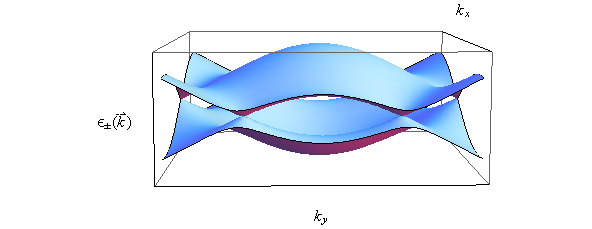
\includegraphics[scale=0.6]{images/tight-binding}}	
				\caption{A three dimensional plot of the full energy spectrum for a hexagonal graphene sheet from Equation (\ref{mod-fk}). This plot clearly shows the Dirac points located at the corners of the Brillouin zone.}
				\label{introduction-fk-plot}
			\end{figure}
%%%%%
%%%%%
%%%%%
		\subsection{Second Nearest Neighbor}
		\label{Introduction - Second Nearest Neighbor}
			To include second nearest neighbor hopping the method is similar and can be taken to be the same until Equation (\ref{introduction-start-tb}). The vector $\vec{R}$ must then be expanded to include the next A lattice atoms and becomes:
			\begin{align}
				\vec{R}=0, \vec{a}_{1}, \vec{a}_{2}, -\vec{a}_{1}, -\vec{a}_{2}, \vec{a}_{1}-\vec{a}_{2}, \vec{a}_{2}-\vec{a}_{2}
			\end{align}
			Evaluating the sum in Equation (\ref{introduction-start-tb}) with the new vector $\vec{R}$:
			\begin{align}
				\langle\varphi_{a}|\psi_{k}\rangle&=b_{a}+b_{b}\alpha f\left(\vec{k}\right)+b_{a}\alpha_{2}\left(e^{i\vec{k}\cdot\vec{a}_{1}}+e^{i\vec{k}\cdot\vec{a}_{2}}+e^{-i\vec{k}\cdot\vec{a}_{1}}+e^{-i\vec{k}\cdot\vec{a}_{2}}+e^{i\vec{k}\cdot\left(\vec{a}_{1}-\vec{a}_{2}\right)}+e^{i\vec{k}\cdot\left(\vec{a}_{2}-\vec{a}_{1}\right)}\right)\\
				&=b_{a}+b_{b}\alpha f\left(\vec{k}\right)+2b_{a}\alpha_{2}\left(\cos\left(\vec{k}\cdot \vec{a}_{1}\right)+\cos\left(\vec{k}\cdot \vec{a}_{2}\right)+\cos\left(\vec{k}\cdot \vec{a}_{1}-\vec{k}\cdot \vec{a}_{2}\right)\right)\\
				&=b_{a}+b_{b}\alpha f\left(\vec{k}\right)+b_{a}\alpha_{2}g\left(\vec{k}\right)
			\end{align}
			Where $g\left(\vec{k}\right)$ has been defined as:
			\begin{align}
				g\left(\vec{k}\right)&=2\left(\cos\left(\vec{k}\cdot \vec{a}_{1}\right)+\cos\left(\vec{k}\cdot \vec{a}_{2}\right)+\cos\left(\vec{k}\cdot \vec{a}_{1}-\vec{k}\cdot \vec{a}_{2}\right)\right)\\
				&=2\cos\left(\sqrt{3}ak_{y}\right)+4\cos\left(\frac{3}{2}ak_{x}\right)\cos\left(\frac{\sqrt{3}}{2}ak_{y}\right)
			\end{align}
			and:
			\begin{align}
				\alpha_{2}=\int\varphi^{*}\left(\vec{r}\right)\varphi\left(\vec{r}+\vec{a}_{1,2}\right)d\vec{r}
			\end{align}
			Then with Equation (\ref{introduction-start-tb-b}), the new vector $\vec{R}$ centered at a B site will find all second nearest neighbors and therefore is the same as the A site, so evaluating the sum:
			\begin{align}
				\langle\varphi_{b}|\psi_{k}\rangle=b_{b}+b_{a}\alpha f^{*}\left(\vec{k}\right)+b_{b}\alpha_{2}g\left(\vec{k}\right)
			\end{align}
			Then evaluating $\langle\varphi_{a,b}|\Delta u|\psi_{k}\rangle$:
			\begin{align}
				\langle\varphi_{a}|\Delta u|\psi_{k}\rangle&=b_{a}\beta+b_{b}tf\left(\vec{k}\right)+b_{a}t'g\left(\vec{k}\right)\\
				\langle\varphi_{b}|\Delta u|\psi_{k}\rangle&=b_{b}\beta+b_{a}tf^{*}\left(\vec{k}\right)+b_{b}t'g\left(\vec{k}\right)
			\end{align}
			with the definition:
			\begin{align}
				t'\equiv\int\varphi^{*}\left(\vec{r}\right)\Delta u\left(\vec{r}\right)\varphi\left(\vec{r}+\vec{a}_{1,2}\right) d\vec{r}
			\end{align}
			The total energy of the system, including hopping from second nearest neighbors can now be written as a set of simultaneous equations:
			\begin{align}
				b_{a}\left(\varepsilon_{k}+\varepsilon_{k}\alpha_{2}g\left(\vec{k}\right)-E-\alpha_{2}g\left(\vec{k}\right)-\beta-t'g\left(\vec{k}\right)\right)+b_{b}f\left(\vec{k}\right)\left(\varepsilon_{k}\alpha-E\alpha-t\right)&=0\\
				b_{a}f^{*}\left(\vec{k}\right)\left(\varepsilon_{k}\alpha-E\alpha-t\right)+b_{b}\left(\varepsilon_{k}+\varepsilon_{k}\alpha_{2}g\left(\vec{k}\right)-E-\alpha_{2}g\left(\vec{k}\right)-\beta-t'g\left(\vec{k}\right)\right)&=0
			\end{align}
			Due to similar conditions as the nearest neighbor only case; $\alpha=0$, $\alpha_{2}=0$, $E=0$, $\beta=0$. In matrix form these equations become:
			\begin{align}
				\hat{H}=\left[\begin{array}{ccc}
					-\varepsilon_{k}+t'g\left(\vec{k}\right)&t f\left(\vec{k}\right)\\
					t f^{*}\left(\vec{k}\right)&-\varepsilon_{k}+t'g\left(\vec{k}\right)
				\end{array}\right]\hspace{1cm}\det\left(\hat{H}\right)=0
			\end{align}
			Which produces the eigenvalue:
			\begin{align}
				\varepsilon_{\pm}\left(\vec{k}\right)=t'g\left(\vec{k}\right)\pm t\sqrt{3+g\left(\vec{k}\right)}
				\label{fk-second}
			\end{align}
			A plot of this energy spectrum can be seen in Figure \ref{introduction-fk-plot-second}. This plot shows the energy spectrum has become asymmetrical around the Fermi level \cite{b1}, however maintains the Dirac points at the corners of the Brillouin zone.
			\begin{figure}[h]
				\centerline{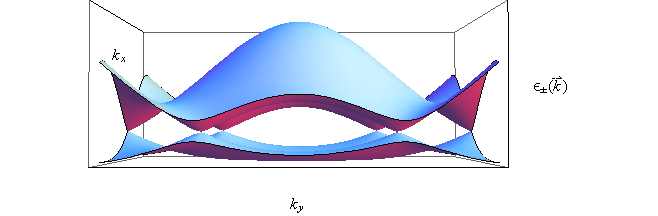
\includegraphics[scale=0.6]{images/tb-second}}
				\caption{A three dimensional plot of the full energy spectrum for a hexagonal graphene sheet from Equation (\ref{fk-second}) including second nearest neighbor hopping. The inclusion of the second nearest neighbor hopping breaks the symmetry for electrons and holes.}
				\label{introduction-fk-plot-second}
			\end{figure}
%%%%%
%%%%%
%%%%%
		\section{Hamiltonian}
		\label{Introduction - Hamiltonian}
			A two variable Taylor expansion around a Dirac point will produce the Hamiltonian for quasiparticles at a Dirac point. This is done by first setting $\vec{k}\rightarrow \vec{k_{2}}+\vec{j}$, where $\vec{k_{2}}$ was derived in Section \ref{Introduction - Zig-Zag Orientation}. With this adjustment the momentum becomes:
			\begin{equation}
				\vec{k}=\left(\frac{2\pi}{3a}+j_{x},\frac{2\pi}{3\sqrt{3}a}+j_{y}\right)
				\label{kpoint}
			\end{equation}
			The full energy spectrum from Section \ref{nearest-neighbor-only} becomes:
			\begin{align}
				f\left(\vec{k}\right)&=1+2e^{-i\left(\frac{3a}{2}\left(k_{x}+j_{x}\right)\right)}\cos\left(\frac{\sqrt{3}a}{2}\left(k_{y}+j_{y}\right)\right)\\
				&=1+2e^{-i\left(\frac{3a}{2}j_{x}\right)}\cos\left(\frac{2\pi}{3}+\frac{\sqrt{3}a}{2}j_{y}\right)\\
				&=1+e^{-i\frac{3a}{2}j_{x}}\left(\cos\left(\frac{\sqrt{3}a}{2}j_{y}\right)-\sqrt{3}\sin\left(\frac{\sqrt{3}a}{2}j_{y}\right)\right)
			\end{align}
			By performing a two variable Taylor expansion around the point $\left(k_{x}, k_{y}\right)$ an approximation of $f(\vec{k})$ and $f^{*}(\vec{k})$ can be made around the region of a Dirac point. The first order, two variable Taylor expansion around point $a$,$b$ is defined as:
			\begin{align}
				f\left(x,y\right)=f\left(a,b\right)+\left(x-a\right)f'_{x}\left(a,b\right)+\left(y-b\right)f'_{y}\left(a,b\right)
			\end{align}
			Applying this to $f\left(k_{x},k_{y}\right)$ produces:
			\begin{align}
				f\left(k_{x},k_{y}\right)&=f\left(j_{x},j_{y}\right)+\left(k_{x}-j_{x}\right)f'_{x}\left(j_{x},j_{y}\right)+\left(k_{y}-j_{y}\right)f'_{y}\left(j_{x},j_{y}\right)\\
				f'_{x}\left(j_{x},j_{y}\right)&=-i\frac{3a}{2}e^{-i\frac{3a}{2}j_{x}}\left(\cos\left(\frac{\sqrt{3}a}{2}j_{y}\right)-\sqrt{3}\sin\left(\frac{\sqrt{3}a}{2}j_{y}\right)\right)\\
				f'_{y}\left(j_{x},j_{y}\right)&=e^{-i\frac{3a}{2}j_{x}}\left(-\frac{\sqrt{3}a}{2}\sin\left(\frac{\sqrt{3}a}{2}j_{y}\right)-\frac{3a}{2}\cos\left(\frac{\sqrt{3}a}{2}j_{y}\right)\right)
			\end{align}
			Setting $\vec{j}=0$  centers the expansion around a Dirac point; $f(\vec{k})$ and $f^{*}(\vec{k})$ become:
			\begin{align}
				f\left(k_{x}, k_{y}\right)=-i\frac{3a}{2}k_{x}-\frac{3a}{2}k_{y}
				\hspace{1cm}
				f^{*}\left(k_{x}, k_{y}\right)=i\frac{3a}{2}k_{x}-\frac{3a}{2}k_{y}
				\label{fofk}
			\end{align}
			These can then be substituted into the whole spectrum to find the Hamiltonian at a Dirac point.
			\begin{align}
				\hat{H}=
				\left[\begin{array}{ccc}
					\varepsilon_{k}&t\left(-i\frac{3a}{2}k_{x}-\frac{3a}{2}k_{y}\right)\\
					t\left(i\frac{3a}{2}k_{x}-\frac{3a}{2}k_{y}\right)&\varepsilon_{k}
				\end{array}\right]
			\end{align}
			$\varepsilon_{k}$ can be set to zero to center the spectrum at the Fermi level. The result here is produced from the vectors in Section \ref{Introduction - Zig-Zag Orientation}, in order to obtain the result for the 2x2 Hamiltonian in \cite{b2,b4} different rotations of the lattice vectors are needed. The standard graphene Hamiltonian is given as:
			\begin{align}
				\hat{H}=v_{f}\sigma_{x,y}\cdot\hat{p}+\sigma_{z}m
				\hspace{1cm}
				v_{f}=\frac{3at}{2\hbar}=\frac{c}{300}
				\hspace{1cm}
				\hat{p}=-i\hbar\bigtriangledown
				\hspace{1cm}
				m=m_{0}v_{f}^{2}
				\label{introduction - hamiltonian eq}
			\end{align}
			Where $a=0.142$ nm \cite{b8}, the hopping energy $t=2.8$ eV \cite{b1}, $m_{0}$ is a mass term \cite{b47} and $c$ is the speed of light in a vacuum. The Hamiltonian can be expanded into matrix form using the Pauli matrices:
			\begin{align}
				\sigma_{x}=
				\left[\begin{array}{ccc}
					0&1\\
					1&0
				\end{array}\right]
				\hspace{1cm}\sigma_{y}=
				\left[\begin{array}{ccc}
					0&-i\\
					i&0
				\end{array}\right]
				\hspace{1cm}\sigma_{z}=
				\left[\begin{array}{ccc}
					1&0\\
					0&-1
				\end{array}\right]
			\end{align}
			and the definition of momentum operator to produce:
			\begin{align}
				\hat{H}=\left[\begin{array}{ccc}
					m&-\hbar v_{f}\left(i\frac{\partial}{\partial x}+\frac{\partial}{\partial y}\right)\\
					-\hbar v_{f}\left(i\frac{\partial}{\partial x}-\frac{\partial}{\partial y}\right)&-m
				\end{array}\right]
			\end{align}
			By using a different Dirac point, known as a $k'$ point instead of Equation (\ref{kpoint}) the two by two Hamiltonian for the $k'$ point can also be found. The two sets of simultaneous equations can then be combined to form the four by four Hamiltonian:
			\begin{align}
				\hat{H}=\hbar v_{f}\left[\begin{array}{cccc}
					m/\hbar v_{f}&k_{x}+ik_{y}&0&0\\
					k_{x}-ik_{y}&-m/\hbar v_{f}&0&0\\
					0&0&-m/\hbar v_{f}&-k_{x}-ik_{y}\\
					0&0&-k_{x}+ik_{y}&m/\hbar v_{f}
				\end{array}\right]
			\end{align}
			This matrix is directly comparable to the Hamiltonian derived from gamma matrices for the Dirac equation or inverted band structure heterojunctions \cite{b41}. This combined with the near relativistic Fermi velocity makes graphene an ideal candidate for use with the Dirac equation for relativistic particles. However since the non-zero sub matricies are essentially negatives of eachother, for simplicity the two by two Hamiltonian is often used. If results for the four by four Hamiltonian are required they are easily obtained from the two by two Hamiltonian.
%%%%%
%%%%%
%%%%%
		\section{Dispersion relation at Dirac points}
		\label{Introduction - Dispersion relation at Dirac points}
			By finding the eigenvalue of the graphene Hamiltonian, the dispersion relation for graphene at a Dirac point can be found.
			\begin{align}
				\det\left(\hat{H}-E\right)=0\hspace{1cm}E=\pm\sqrt{\hbar^{2}v_{f}^{2}\left(k_{x}^{2}+k_{y}^{2}\right)+m^{2}}
				\label{introduction-ekm}
			\end{align}
			This produces a Dirac cone when $m=0$ \cite{b5, b55} showing the conduction and valance band touching at a Dirac point. The energy spectrum with a mass term \cite{b46, b47, b4, b55} becomes parabolic with a gap between the conduction and valance band equivalant to $2m$. This gap may be formed in zig-zag type nanoribbons \cite{b1}, the application of strain \cite{b59}, by interaction with a substrate and by transverse electric field \cite{b47} in situations when inversion symmetry is broken.

			\begin{figure}[h]
				 \begin{subfigure}[h]{0.45\textwidth}
					\centerline{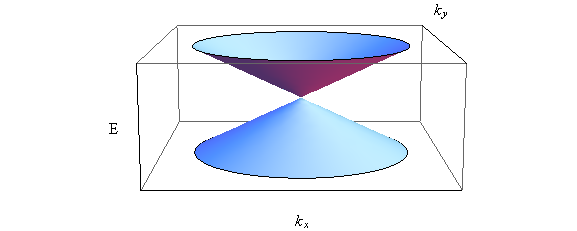
\includegraphics[scale=0.5]{images/dispersion}}
					\caption{$m=0$}
				\end{subfigure}
				\hspace{1cm}
				\begin{subfigure}[h]{0.45\textwidth}
					\centerline{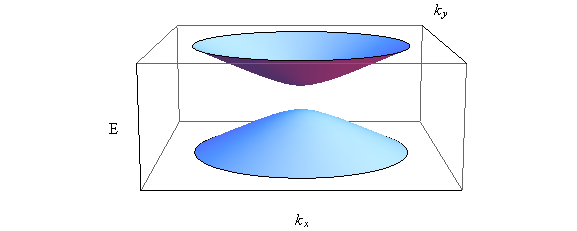
\includegraphics[scale=0.5]{images/dispersion-m}}
					\caption{$m\ne 0$}
				\end{subfigure}
				\caption{The energy momentum relation near a Dirac point from Equation (\ref{introduction-ekm}). In (a) the gapless spectrum shows a Dirac cone with the energy bands touching at a Dirac point. In (b) graphene has a parabolic energy spectrum with an energy gap of $2m$ between the energy bands.}
			\end{figure}
%%%%%
%%%%%
%%%%%
%		\section{Zener Tunnelling}
%		\label{Introduction - Zener Tunnelling}
%The linear dispersion relation that allows for Klein tunnelling through potential barriers also makes graphene an ideal candidate for Zener tunnelling devices. Zener tunnelling is the process whereby an electron may be excited from the valence band into the conduction band by a strong electric field \cite{b42,b43}. In this section the rate at which electrons may jump from the valence band will be determined using the methods outlined in \cite{b42}.
%
%		For a one dimensional lattice, the potential energy of the electron is represented by $V\left(x\right)$ with a period $a$. The wave equation of a periodic potential has solutions in the form of a Bloch wave-function \cite{b44}. 
%		\begin{equation}
%			\psi_{k}=e^{ikx}U_{k}\left(x\right)
%		\end{equation}
%		where the function $U_{k}\left(x\right)$ has the same period as $V\left(x\right)$, $a=2\pi/k$. The condition that the wave-function must be finite for all values of $x$ requires that $k$ is real when the enregy $E_{k}$ is within the allowed energy bands. The periodicity of the wave-function requires that the first energy band lies within the interval $-\pi/a \leq k \leq \pi/a$.
%		If an electric field $F$ is present, the wave-function $\psi\left(x,t\right)$ is expanded in terms of wave-functions of the lowest energy band when $F=0$:
%		\begin{equation}
%			\psi\left(x,t\right)=\int^{\pi/a}_{-\pi/a}g\left(k,t\right)\psi_{k}dk
%		\end{equation}
%		If transitions are only allowed for the first of each energy band the continuity equation:
%		\begin{equation}
%			\frac{d}{dt}|g|^{2}+\frac{2\pi eF}{h}|g|^{2}=0
%		\end{equation}
%		requires that $|g|^{2}$ is a function of $k$ and $t$ so that:
%		\begin{equation}
%			|g|^{2}=G\left(k-\frac{2\pi eF}{h}t\right)
%		\end{equation}
%		where $G$ is an arbitary function. With the periodic boundary of $\psi_{-\pi/a}=\psi_{\pi/a}$, $|g|^{2}$ must also be periodic with $t$. The frequency can then be calculated from $f=v/\lambda$ where:
%		\begin{align}
%			\lambda=\frac{2\pi}{a}\hspace{1cm}v=\frac{2\pi eF}{h}\hspace{1cm}f=\frac{eFa}{h}
%		\end{align}
%		To calculate the probability per unit time $\gamma$, that an electron will be excited into the conduction band the frequency of the wave packet must be multiplied by the probability of tunelling $p$.
%		\begin{equation}
%			\gamma = fp
%		\end{equation}
%		In order to calculate $p$, a wave-function periodic in time can be use with the wave equation:
%		\begin{equation}
%			\left(\frac{h^{2}}{8\pi^{2}m}\frac{d^{2}}{dx^{2}}-V\left(x\right)+\left(E-eFx\right)\right)\psi=0
%			\label{zener-wave}
%		\end{equation}
%		Assuming that $eFx$ does not vary much between atoms, the solution can be chosen to be in the form of:
%		\begin{equation}
%			\psi=e^{i\int K dx}U_{K}\left(x\right)
%			\label{zener-psi}
%		\end{equation}
%		where $K$ is a function of $\left(E-eFx\right)$ and $U_{K}$ is identical to the previous $U_{k}$ with $k=K$. With this defintion, $K$ will only become real with certain values of $E$ and $x$. If $K$ becomes imaginary the wave-function in Equation.(\ref{zener-psi}) will begin to decay. In each allowed energy band in Figure \ref{zener-flat} the wave-functions for electrons should be in the same oscillatory form, with decaying probability in the gap region. With oscillatory wave-functions in regions AB, CD and decaying wave-functions in region BC the transition probability $p$ between bands is given as:
%		\begin{equation}
%			p=|\psi_{CD}/\psi_{AB}|^{2}
%		\end{equation}
%
%\begin{figure}
%	\centerline{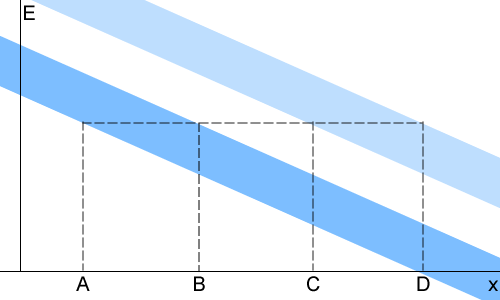
\includegraphics[scale=0.6]{images/zener-flat}}
%	\caption{Diagram of energy bands in a dielectric material in an electric field. The valence band (dark) and conduction band (light) are separated by a forbidden energy gap.}
%	\label{zener-flat}
%\end{figure}
%		
%		To allow Equation.(\ref{zener-psi}) to be either oscillatory or decaying, $K$ can be expressed as it's real and imaginary components:
%		\begin{equation}
%			K=\xi\left(x\right)+i\eta\left(x\right)
%		\end{equation}
%		As the wave-function must decay within the disallowed region, the probability must be in the form of exponential decay within region BC. This results in the probability:
%		\begin{equation}
%			|\psi_{CD}/\psi_{AB}|=e^{-\int^{C}_{B}\eta\left(x\right)dx}
%		\end{equation}
%		and the probability per unit time is then:
%		\begin{equation}
%			\gamma=\frac{eFa}{h}e^{-2\int^{C}_{B}\eta\left(x\right)dx}
%			\label{zener-gamma}
%		\end{equation}
%		To obtain an expression for $K$, the wave equation can be expressed as Hill's equation, in general form:
%		\begin{equation}
%			\frac{d^{2}}{dx^{2}}\psi+\left(\theta_{0}+2\Sigma_{n}\theta_{n}cos\left(2nx\right)\right)\psi=0
%		\end{equation}
%		This can be constructed with the substitutions $s=\pi x/a$ and $\theta_{0}=8ma^{2}(E-eFx)/h^{2}$ to Equation.(\ref{zener-wave}), resulting in:
%		\begin{equation}
%			\frac{d^{2}}{ds^{2}}\psi+\left(\theta_{0}+\frac{8ma^{2}}{h^{2}}V\left(x\right)\right)\psi=0
%		\end{equation}
%		The remaining terms are obtained by a Fourier series of $V(x)$. The Fourier series is defined as:
%		\begin{equation}
%			f\left(x\right)=\frac{1}{2}a_{0}+\sum\limits_{n=1}^{\infty}a_{a}cos\left(nx\right)+\sum\limits_{n=1}^{\infty}b_{n}sin\left(nx\right)
%		\end{equation}
%		where:
%		\begin{align}
%			a_{0}&=\frac{1}{\pi}\int^{\pi}_{-\pi}f\left(x\right)dx\\
%			a_{n}&=\frac{1}{\pi}\int^{\pi}_{-\pi}f\left(x\right)cos\left(nx\right)dx\\
%			b_{n}&=\frac{1}{\pi}\int^{\pi}_{-\pi}f\left(x\right)sin\left(nx\right)dx
%		\end{align}
%		As $V(x)$ must be a periodic function, the integration rules:
%		\begin{align}
%			&\int^{\pi}_{-\pi}sin\left(mx\right)sin\left(nx\right)dx=\pi \delta_{mn}
%			\hspace{1cm}			
%			&&\int^{\pi}_{-\pi}cos\left(mx\right)cos\left(nx\right)dx=\pi \delta_{mn}\\
%			&\int^{\pi}_{-\pi}cos\left(mx\right)sin\left(nx\right)dx=0
%			\hspace{1cm}
%			&&\int^{\pi}_{-\pi}sin\left(mx\right)cos\left(nx\right)dx=0\\
%			&\int^{\pi}_{-\pi}cos\left(mx\right)dx=0
%			\hspace{1cm}
%			&&\int^{\pi}_{-\pi}sin\left(mx\right)dx=0
%		\end{align}
%		can be used, with a potential of form $V(x)=cos(nx)$ with $x=sa/\pi$ and $a=2\pi$ to produce the equation:
%		\begin{equation}
%			\frac{d^{2}}{ds^{2}}\psi+\left(\theta_{0}+2\Sigma_{n}\theta_{m}cos\left(2ns\right)\right)\psi=0
%			\label{zener-hill}
%		\end{equation}
%		Where $\theta_{m}=4ma^{2}/h^{2}\theta_{n}$ from the fourier expansion. From the solution of Equation.(\ref{zener-hill}) in \cite{b45} the value of $K$ can be expressed in the form:
%		\begin{equation}
%			sin^{2}\left(aK/2\right)=sin^{2}\left(\frac{1}{2}\pi\sqrt{\theta_{0}}\right)\left(1+\frac{\pi\theta_{1}^{2}}{4\sqrt{\theta_{0}}\left(1-\theta_{0}\right)}cot\left(\pi\sqrt{\theta_{0}}/2\right)\right)+O\left(\theta_{1}^{4}\right)
%			\label{zener-hill-result}
%		\end{equation}
%		In the energy region that produces an imaginary $K$, $\theta_{0}$ will only be close to one and therefore $K$ will be approximately equal to $\pi\theta_{0}^{\frac{1}{2}}/2$ or $\pi/2$. With these conditions, the values:
%		\begin{align}
%			\theta_{0}&=1+\alpha \\
%			K&=\pi/2 + \beta
%		\end{align}
%		can be set, where $\alpha$ and $\beta$ are a small deviation. Using these values for $K$ and $\theta_{0}$ with Equation.(\ref{zener-hill-result}) produces the result for $K$:
%		\begin{equation}
%			K=\pi/a \pm i\left(\pi/a\right)\sqrt{\theta_{1}^{2}-\alpha^{2}}
%		\end{equation}
%		With the axis origin set between the points B and C, $K$ can be expressed as:
%		\begin{equation}
%			K=\frac{\pi}{a}\left(1\pm i\frac{8ma^{2}}{h^{2}}\left(V_{0}^{2}-\left(eFx\right)^{2}\right)^{\frac{1}{2}}\right)
%		\end{equation}
%		then with the integration in Equation.(\ref{zener-gamma}) between the points $B=V_{0}/eF$ and $C=-V_{0}/eF$ the rate of transmission becomes:
%		\begin{equation}
%			\gamma=\frac{eFa}{h}e^{-\frac{\pi^{2}}{h^{2}}\frac{ma\epsilon^{2}}{|eF|}}
%		\end{equation}
%		Where the size of the energy gap $\epsilon=2V_{0}$.
%%%%%
%%%%%
%%%%%

	\section{Wave-functions}
	\label{Wave-functions}
		The eigenvectors of the matrix Hamiltonian in Equation (\ref{introduction - hamiltonian eq}) can be used as the wave-functions for quasiparticles in graphene. In this section two types of wave-function will be derived. The oscillatory type wave-function is of the form of a plane wave and is useful for finding the properties of scattering devices. The other type of wave-function derived here is of the form of exponential growth or decay. These wave-functions are useful for finding localised states, where the particle is restricted to a specific region.
			\subsection{Oscillatory}
			\label{Wave-functions - Oscillitary}
			By applying the Hamiltonian to the Dirac equation wave-functions can be found for an infinite graphene sheet. With a potential and an energy gap the time independent Dirac equation takes the form:
			\begin{align}
				\left[\begin{array}{ccc}
				V-E+m&v_{f}\left(\hat{p}_{x}+i\hat{p}_{y}\right)\\
				v_{f}\left(\hat{p}_{x}-i\hat{p}_{y}\right)&V-E-m
				\end{array}\right]
				\left[\begin{array}{ccc}
				\psi_a\\
				\psi_b
				\end{array}\right]
				=0
			\end{align}
			To find non-trivial solutions, this can then be split into a system of simultaneous equations:
			\begin{equation}\label{eq:4}
				\left(V-E+m\right)\psi_{a}+ v_{f}\left(\hat{p}_{x}+i\hat{p}_{y}\right)\psi_{b}=0
			\end{equation}
			\begin{equation}\label{eq:5}
				\left(V-E-m\right)\psi_{b}+v_{f}\left(\hat{p}_{x}-i\hat{p}_{y}\right)\psi_{a}=0
			\end{equation}
			By making $\psi_{b}$ the subject of Equation (\ref{eq:5}), Equation (\ref{eq:4}) can take the form:
			\begin{equation}
				\frac{\left(E-V\right)^{2}-m^{2}}{\hbar^{2}v_{f}^{2}}\psi_{a}=\left(-\frac{\partial^{2}}{\partial x^{2}}-\frac{\partial^{2}}{\partial y^{2}}\right)\psi_{a}
				\label{eq:6}
			\end{equation}
			Since $V=V(x)$ and is independent of $y$, one can look for separable solutions $\psi_{a}(x,y)=f(x)g(y)$. Equation (\ref{eq:6}) then becomes:
			\begin{equation}
				\frac{1}{g(y)}\frac{d^{2}}{dy^{2}}g(y)=-\frac{\left(E-V\right)^{2}-m^{2}}{\hbar^{2}v_{f}^{2}}-\frac{1}{f(x)}\frac{d^{2}}{dx^{2}}f(x).
			\end{equation}
			%Requiring the wave-functions are separable means the wave-functions should be of the form $f\left(x\right)e^{ik_{y}y}$. Evaluating the derivitives with respect to $y$ produces the equation:
			Looking for plane wave solutions $g(y)\sim e^{ik_{y}y}$ gives 
			\begin{equation}
				q^{2}f\left(x\right)=-\frac{d^{2}}{d x^{2}}f\left(x\right),
			\end{equation}
			with the definition:
			\begin{equation}
				q^{2}=\frac{\left(E-V\right)^{2}-m^{2}}{\hbar^{2}v_{f}^{2}}-k_{y}^{2}
			\end{equation}
			A suitable solution of this equation produces the wave-function component:
			\begin{equation}
				\psi_{a}\left(x,y\right)=\left(a_{1}e^{iqx}+a_{2}e^{-iqx}\right)e^{ik_{y}y}
			\end{equation}
			Using the value for $\psi_{a}$, the wave-function component $\psi_{b}$ can be found with Equation (\ref{eq:5}):
			\begin{equation}
				\psi_{b}=\frac{\hbar v_{f}}{E-V+m}\left(-i\frac{\partial}{\partial x}+\frac{\partial}{\partial y}\right)\left(a_{1}e^{iqx}+a_{2}e^{-iqx}\right)e^{ik_{y}y}
			\end{equation}
			Evaluating this with:
			\begin{align}
				q=|\vec{q}|\cos(\theta)
				\hspace{1cm}
				k_{y}=|\vec{q}|\sin(\theta)\hspace{1cm}|\vec{q}|=\sqrt{q^{2}+k_{y}^{2}}=\sqrt{\frac{\left(E-V\right)^{2}-m^{2}}{\hbar^{2}v_{f}^{2}}}
			\end{align}
			Results in the final form of the wave-function component:
			\begin{equation}
				\psi_{b}=\alpha\left(a_{1} e^{iqx+i\theta}-a_{2} e^{-iqx-i\theta}\right)e^{ik_{y}y}
			\end{equation}
			Where constants have been grouped so that:
			\begin{align}
				\alpha=\frac{\sqrt{\left(E-V\right)^{2}-m^{2}}}{E-V+m}
			\end{align}
			Finally with normalisation the wave-functions for graphene with an energy gap and a potential can be stated to be:
			\begin{align}
				\psi\left(x,y\right)=
				c_{n}e^{ik_{y}y}
				\left[\begin{array}{ccc}
					e^{iqx}&e^{-iqx}\\
					\alpha e^{iqx+i\theta}&-\alpha e^{-iqx-i\theta}
				\end{array}\right]
				\left[\begin{array}{ccc}
					a_{1}\\
					a_{2}
				\end{array}\right]
				\label{introduction-wf}
			\end{align}
			where the normalisation constants have been grouped so that $c_{n}=1/\sqrt{1+\alpha^{2}}$. Removing the energy gap from this wave-function produces the known wave-functions for a graphene sheet in \cite{b12}. The validity of these wave-functions can then be tested by inserting them into the time independent Dirac equation.
			\begin{align}
				\hat{H}\psi =E\psi
			\end{align}
			\begin{equation}\label{eq:61}
				\left(V-E+m\right)\left(a_{1}e^{iqx}+a_{2}e^{-iqx}\right)e^{ik_{y}y}-\hbar v_{f}\left(i\frac{\partial}{\partial x}+\frac{\partial}{\partial y}\right)\alpha\left(a_{1}e^{iqx+i\theta}-a_{2}e^{-iqx-i\theta}\right)e^{ik_{y}y}=0
			\end{equation}
			\begin{equation}\label{eq:7}
				\left(V-E-m\right)\alpha\left(a_{1}e^{iqx+i\theta}-a_{2}e^{-iqx-i\theta}\right)e^{ik_{y}y}-\hbar v_{f}\left(i\frac{\partial}{\partial x}-\frac{\partial}{\partial y}\right)\left(a_{1}e^{iqx}+a_{2}e^{-iqx}\right)e^{ik_{y}y}=0
			\end{equation}
			Evaluating Equation (\ref{eq:61}) and expressing $\theta$ in terms of $q$ and $k_{y}$:
			\begin{equation}
				\left(V-E+m\right)\left(a_{1}e^{iqx}+a_{2}e^{-iqx}\right)e^{ik_{y}y}+\frac{\hbar v_{f}\alpha}{|\vec{q}|}\left(q^{2}+k_{y}^{2}\right)\left(a_{1}e^{iqx}+a_{2}e^{-iqx}\right)e^{ik_{y}y}=0
			\end{equation}
			Which simplifies to:
			\begin{equation}
				-\left(E-V\right)^{2}+m^{2}+\left(E-V\right)^{2}-m^{2}=0
			\end{equation}
			Therefore this part satisfies the Dirac equation. The same can now be done to Equation (\ref{eq:7}).
			\begin{align}
				\hbar v_{f}\left(-\left(q+ik_{y}\right)a_{1}e^{iqx}\right. &+ \left. \left(q-ik_{y}\right)a_{2}e^{-iqx}\right)e^{ik_{y}y}\\
				&+\hbar v_{f}\left(\left(q+ik_{y}\right)a_{1}e^{iqx}+\left(-q+ik_{y}\right)a_{2}e^{-iqx}\right)e^{ik_{y}y}=0
			\end{align}
			Hence these wave-functions satisfy the Dirac equation and can be used in the further analysis of graphene systems. These wave-functions have been plotted with respect to the $x$ direction in Figure \ref{oscillitary-psi-a}. This plot shows the oscillatory form of the wave-function and the $\psi_{b}$ component is shifted by the phase change $\theta$.
\begin{figure}
	\begin{subfigure}{0.45\textwidth}
		\centerline{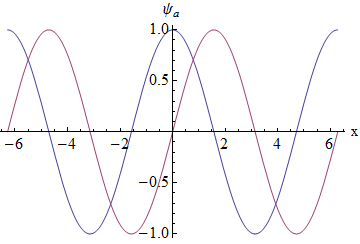
\includegraphics[scale=0.6]{images/oscillitary-psi-a}}
		\caption{$\psi_{a}$}
		\label{}
	\end{subfigure}
	\hspace{1.2cm}
	\begin{subfigure}{0.45\textwidth}
		\centerline{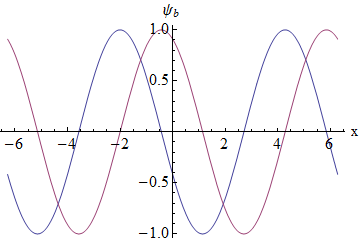
\includegraphics[scale=0.6]{images/oscillitary-psi-b}}
		\caption{$\psi_{b}$}
		\label{}
	\end{subfigure}
	\caption{Example plots of wave-function against spacial direction from Equation (\ref{introduction-wf}). Here oscillatory wave-functions are shown where the blue curves are the real component and the red curves are the imaginary component. The $\psi_{a}$ component of the graphene wave-function is shown in (a) and the $\psi_{b}$ component is shown in (b).}
	\label{oscillitary-psi-a}
\end{figure}
%%%%%
%%%%%
%%%%%
			\subsection{Growth and Decay}
			\label{Wave-functions - Growth and Decay}
				Here wave-functions which display exponential growth and decay are found. These will be useful for calculating bound states. By requiring that $\psi_{a}$ is of the form:
				\begin{align}
					\psi_{a}=\left(a_{1}e^{q_{d}x}+a_{2}e^{-q_{d}x}\right)e^{ik_{y}y}
				\end{align}
				$\psi_{b}$ can be found from the graphene Hamiltonian.
				\begin{align}
					\psi_{b}&=\frac{\hbar v_{f}}{V-E-m}\left(i\frac{\partial}{\partial x}-\frac{\partial}{\partial y}\right)\psi_{a}
				\end{align}
				Evaluating this shows:
				\begin{align}
					\psi_{b}=i\left(a_{1}\alpha_{-}e^{q_{d}x}-a_{2}\alpha_{+}e^{-q_{d}x}\right)e^{ik_{y}y}
				\end{align}
				With the group of constants defined as:
				\begin{align}
					\alpha_{\pm}=\frac{\hbar v_{f}}{V-E-m}\left(q_{d}\pm k_{y}\right)
				\end{align}
				The wave-functions should then be inserted into the Dirac equation to check validity.
				\begin{align}
					\hat{H}\psi=E\psi
				\end{align}
				\begin{align}
					\left[\begin{array}{ccc}
						V-E+m&-\hbar v_{f}\left(i\frac{\partial}{\partial x}+\frac{\partial}{\partial y}\right)\\
						-\hbar v_{f}\left(i\frac{\partial}{\partial x}-\frac{\partial}{\partial y}\right)&V-E-m
					\end{array}\right]
					\left[\begin{array}{ccc}
						a_{1}e^{q_{d}x}+a_{2}e^{-q_{d}x}\\
						i\left(\alpha_{-}a_{1}e^{q_{d}x}-\alpha_{+}a_{2}e^{-q_{d}x}\right)
					\end{array}\right]e^{ik_{y}y}
					=0
				\end{align}
				This provides the two equations:
				\begin{align}
					\left(V-E+m\right)\left(a_{1}e^{q_{d}x}\right. &+ \left.a_{2}e^{-q_{d}x}\right)e^{ik_{y}y}\\
					&-\hbar v_{f}\left(i\frac{\partial}{\partial x}+\frac{\partial}{\partial y}\right)\left(\alpha_{-}a_{1}e^{q_{d}x}-\alpha_{+}a_{2}e^{-q_{d}x}\right)e^{ik_{y}y}=0
				\end{align}
				\begin{align}
					-\hbar v_{f}\left(i\frac{\partial}{\partial x}-\frac{\partial}{\partial y}\right)\left(a_{1}e^{q_{d}x}\right. &+ \left. a_{2}e^{-q_{d}x}\right)e^{ik_{y}y}\\
					&+i\left(V-E-m\right)\left(\alpha_{-}a_{1}e^{q_{d}x}-\alpha_{+}a_{2}e^{-q_{d}x}\right)e^{ik_{y}y}=0
				\end{align}
				Which show that:
				\begin{align}
					q_{d}=\sqrt{k_{y}^{2}-\frac{\left(E-V\right)^{2}+m^{2}}{\hbar^{2}v_{f}^{2}}}
				\end{align}
				With this value of $q_{d}$ the wave-functions satisfy the Dirac equation so the wave-functions can finally take the form:
				\begin{align}
					\psi=e^{ik_{y}y}
					\left[\begin{array}{ccc}
						e^{q_{d}x}&e^{-q_{d}x}\\
						i\alpha_{-}e^{q_{d}x}&-i\alpha_{+}e^{-q_{d}x}
					\end{array}\right]
					\left[\begin{array}{ccc}
						a_{1}\\
						a_{2}
					\end{array}\right]
					\label{introduction-wf-gd}
				\end{align}
				With $m=0$ these wave-functions match the wave-functions in \cite{b3}. The exponential growth wave-functions have been plotted in Figure \ref{growth-psi-a}. This plot shows that both the $\psi_{a}$ and $\psi_{b}$ terms are exponentially growing with real only components in $\psi_{a}$ and imaginary only components in $\psi_{b}$. As with the oscillatory case the $\psi_{b}$ component experiences a phase shift.
\begin{figure}
	\begin{subfigure}{0.45\textwidth}
		\centerline{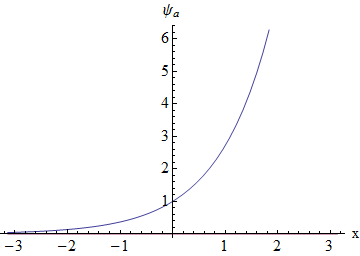
\includegraphics[scale=0.6]{images/growth-psi-a}}
		\caption{$\psi_{a}$}
		\label{}
	\end{subfigure}
	\hspace{1.2cm}
	\begin{subfigure}{0.45\textwidth}
		\centerline{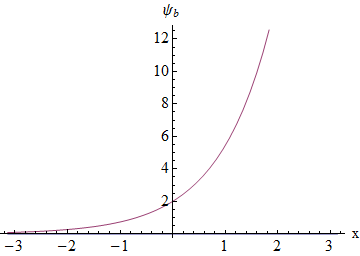
\includegraphics[scale=0.6]{images/growth-psi-b}}
		\caption{$\psi_{b}$}
		\label{}
	\end{subfigure}
	\caption{Example plots of wave-function against spacial direction from Equation (\ref{introduction-wf-gd}). Here exponential growth wave-functions are shown where the blue curves are the real component and the red curves are the imaginary component. The $\psi_{a}$ component of the graphene wave-function is shown in (a) and the $\psi_{b}$ component is shown in (b).}
	\label{growth-psi-a}
\end{figure}
%%%%%
%%%%%
%%%%%
	\section{Magnetic Field}
		\label{Introduction - Magnetic Field}
		In this section the properties of infinite sheet graphene will be examined with an external perpendicular magnetic field applied to it. The momentum must be modified to account for the contributions from the magnetic field by the Peierls substitution \cite{b39}. In a magnetic field the linear energy-momentum relation will be replaced by energy levels. These energy levels will be obtained using the modified graphene Hamiltonian for magnetic field. Finally this Hamiltonian will be used to obtain wave-functions for charge carriers in an infinite sheet of graphene with an external magnetic field.
		\subsection{Peierls Substitution}
			The Peierls substitution changes the expression for momentum to allow for an external magnetic field. To do this a charged particle of charge $q$ can be considered. When a charged particle moves though a magnetic field, the Lorentz force associated with this particle is:
			\begin{equation}
				\vec{F}=q\left(\vec{E}+\vec{v}\times \vec{B}\right)
			\end{equation}
			Where the electric and magnetic field strengths are defined as:
			\begin{align}
			\vec{B}=\bigtriangledown \times \vec{A}\hspace{1cm}\vec{E}=-\bigtriangledown\phi-\frac{d\vec{A}}{dt}
			\end{align}
			Substituting these definitions into the Lorentz force provides:
			\begin{equation}
				\vec{F}=q\left(-\bigtriangledown\phi-\frac{d\vec{A}}{dt}+\bigtriangledown\left(\vec{v}\cdot\vec{A}\right)\right)
			\end{equation}
			The force is related to potential energy by:
			\begin{align}
				\vec{F}=-\bigtriangledown V\left(\vec{r}\right)\hspace{1cm}V\left(\vec{r}\right)=-\int\vec{F}d\vec{r}
			\end{align}
			Converting the force into a potential and with the condition $d\vec{A}/dt=0$ for a conservative field, results in the potential:
			\begin{equation}
				V\left(\vec{r}\right)=q\left(\phi-\vec{v}\cdot\vec{A}\right)
				\label{peierl-v}
			\end{equation}
			The Lagrangian is defined as:
			\begin{equation}
				L=T-V
			\end{equation}
			Where $T$ is the kinetic energy and $V$ is the potential energy. With the general definition of kinetic energy and potential energy from Equation (\ref{peierl-v}):
			\begin{equation}
				L=\frac{1}{2}m\vec{v}^{2}-q\phi+\frac{q}{c}\vec{v}\cdot\vec{A}
				\label{peierl-L}
			\end{equation}
			To find the momentum from the Lagrangian:
			\begin{equation}
				\frac{dL}{d\vec{v}}=\vec{p}=m\vec{v}+q\vec{A}
				\label{lagrangian momentum}
			\end{equation}
			Using definitions of the Hamiltonian and Lagrangian, the Hamiltonian can be obtained form the Langrangian with the relation:
			\begin{equation}
				H=T+V=2T-L=\vec{v}\cdot\vec{p}-L
			\end{equation}
			With the definition of the Lagrangian from Equation (\ref{peierl-L}):
			\begin{align}
				H&=\vec{v}\cdot\left(m\vec{v}+q\vec{A}\right)-\frac{1}{2}m\vec{v}^{2}+q\phi-q\vec{v}\cdot\vec{A}\\
				&=\frac{1}{2}m\vec{v}^{2}+q\phi
			\end{align}
			The velocity can be expressed as momentum from Equation (\ref{lagrangian momentum}):
			\begin{equation}
				\vec{v}=\frac{1}{m}\left(\vec{p}-q\vec{A}\right)
			\end{equation}
			Resulting in the Hamiltonian:
			\begin{equation}
				H=\frac{1}{2m}\left(\vec{p}-q\vec{A}\right)^{2}+q\phi
			\end{equation}
			The Peierls substitution for momentum in a magnetic field becomes \cite{b39}:
			\begin{equation}
				\vec{p}\rightarrow \vec{p}-q\vec{A}
			\end{equation}
			This substitution for momentum in a magnetic field may also be refered to as canonical momentum.
%%%%%
%%%%%
%%%%%
		\subsection{Landau Levels}
			Under a magnetic field the linear energy-momentum relation is replaced by energy levels \cite{b33}. The Landau levels for graphene in a magnetic field can be derived by using Peierls substitution. The uniform magnetic field is introduced in the $z$ direction.
			\begin{align}
				\hat{H}=v_{f}\sigma \hat{p}
				\hspace{1cm}
				\hat{p}\rightarrow \hat{p}+e\vec{A}
				\hspace{1cm}
				l_{b}=\sqrt{\frac{\hbar}{eB_{0}}}
				\hspace{1cm}
				\vec{B}=
				\left[\begin{array}{ccc}
					0\\
					0\\
					B_{0}
				\end{array}\right]
				\hspace{1cm}
				\vec{A}=B_{0}
				\left[\begin{array}{ccc}
					0\\
					x\\
					0
				\end{array}\right]
			\end{align}
			Using the secular equation $\det\left(\hat{H}-E\right)=0$ produces:
			\begin{equation}
				\frac{E^{2}}{v_{f}^{2}}-\left(\hat{p}_{x}+i\hat{p}_{y}+\frac{i\hbar x}{ l_{b}^{2}}\right)\left(\hat{p}_{x}-i\hat{p}_{y}-\frac{i\hbar x}{ l_{b}^{2}}\right)=0
			\end{equation}
			With the commutation relations:
			\begin{equation}
				\left[\hat{p}_{x},\hat{p}_{y}\right]=0\hspace{1cm}\left[\hat{p}_{x},\hat{x}\right]=-i\hbar
			\end{equation}
			This equation can act on a wave-function with the form $\psi_{a}=f(x)e^{ik_{y}y}$ to replace the $y$ momentum with the corresponding eigenvalue. The equation:
			\begin{equation}
				\left[\frac{E^{2}}{v_{f}^{2}}-\left(\hat{p}_{x}+i\hat{p}_{y}+\frac{i\hbar x}{ l_{b}^{2}}\right)\left(\hat{p}_{x}-i\hat{p}_{y}-\frac{i\hbar x}{ l_{b}^{2}}\right)\right]\psi_{a}=0
			\end{equation}
			can be reduced to:
			\begin{equation}
				\frac{l_{b}^{2}}{\hbar^{2}v_{f}^{2}}E^{2}+1-\frac{l_{b}^{2}}{\hbar^{2}}\hat{p}_{x}^{2}-\frac{1}{l_{b}^{2}}\left(x+l_{b}^{2}k_{y}\right)^{2}=0
				\label{introduction-mag-int}
			\end{equation}
			With the additional substitutions:
			\begin{equation}
				\varepsilon=E^{2}+\frac{\hbar^{2}v_{f}^{2}}{l_{b}^{2}}\hspace{1cm}{\bar x}=x+l_{b}^{2}k_{y}
			\end{equation}
			Equation (\ref{introduction-mag-int}) can be written as:
			\begin{equation}
				\frac{l_{b}^{2}}{\hbar^{2}v_{f}^{2}}\varepsilon-\frac{l_{b}^{2}}{\hbar^{2}}\hat{p}_{x}^{2}-\frac{1}{l_{b}^{2}}{\bar x}^{2}=0
			\end{equation}
			Which can be matched to the quantum harmonic oscillator derived in Section \ref{Appendix - Quantum Harmonic Oscillator}:
			\begin{equation}
				2mE-\hat{p}_{x}^{2}-m^{2}\omega^{2}x^{2}=0
			\end{equation}
			Then by analogy:
			\begin{equation}
				2m=\frac{l_{b}^{2}}{\hbar^{2}v_{f}^{2}}\hspace{1cm}1=\frac{\hbar^{2}}{l_{b}^{2}}\hspace{1cm}m^{2}\omega^{2}=\frac{1}{l_{b}^{2}}\hspace{1cm}\omega=2\frac{\hbar v_{f}^{2}}{l_{b}^{2}}
			\end{equation}
			The known result for the quantum harmonic oscillator $E_{n}=\hbar\omega\left(n+1/2\right)$ can be converted to the graphene case, resulting in \cite{b37, b53}:
			\begin{equation}
				E_{n}=\pm \frac{\hbar v_{f}}{l_{b}}\sqrt{2n}
				\label{landau-levels-e}
			\end{equation}
			If an external potential and constant energy gap are introduced into the graphene Hamiltonian the Landau levels change to:
			\begin{equation}
				E_{n}=V \pm \frac{\hbar v_{f}}{l_{b}}\sqrt{\frac{l_{b}^{2}}{\hbar^{2}v_{f}^{2}}m^{2}+2n}
				\label{landau-levels-e-m}
			\end{equation}

			In Figure \ref{landau-levels} the first five Landau levels are shown with their dependencies on the magnetic length $l_{b}$. In Figure \ref{landau-levels} (b) an energy gap and external potential have been included. The energy gap increase the gap between the first energy level, which in turn causes the energy levels to be found closer to eachother. The external potential shifts the levels in the energy axis.
			\begin{figure}
				\begin{subfigure}{0.45\textwidth}
					\centerline{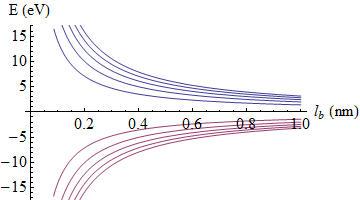
\includegraphics[scale=0.6]{images/landau-levels}}
					\caption{$V=0$ eV and $m=0$ eV.}
				\end{subfigure}
				\hspace{1.2cm}
				\begin{subfigure}{0.45\textwidth}
					\centerline{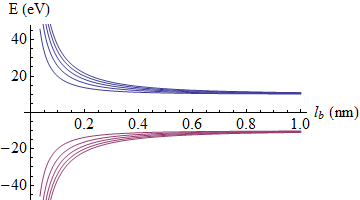
\includegraphics[scale=0.6]{images/landau-levels-v-m}}
					\caption{$V=5$ eV and $m=5$ eV.}
				\end{subfigure}
				\caption{Plot showing the first five Landau levels and their dependence on magnetic length $l_{b}$ from Equation (\ref{landau-levels-e}) and Equation (\ref{landau-levels-e-m}). Here $\hbar v_{f}$ has been taken to be equal to one.}
				\label{landau-levels}
			\end{figure}

%%%%%
%%%%%
%%%%%
			\subsection{Wave-functions}
			\label{Wave-functions - Magnetic Field}
				The wave-functions for graphene in a magnetic field can be derived from the graphene Hamiltonian with Peierls substitution.
				\begin{align}
					\hat{H}=v_{f}\sigma \hat{p}+IV+\sigma_{z}m\hspace{1cm}\hat{p}\rightarrow \hat{p}+e\vec{A}
				\end{align}
				With an external magnetic field in the $z$ direction and the Landau gauge:
				\begin{align}
					l_{b}=\sqrt{\frac{\hbar}{eB_{0}}}
					\hspace{1cm}\vec{B}=
					\left[\begin{array}{ccc}
						0\\
						0\\	
						B_{0}
					\end{array}\right]
					\hspace{1cm}\vec{A}=B_{0}
					\left[\begin{array}{ccc}
						0\\
						x\\
						0
					\end{array}\right]
					\hspace{1cm}I=\left[\begin{array}{ccc}
						1 & 0\\
						0 & 1
					\end{array}\right]
				\end{align}
				The time independent Dirac equation becomes:
				\begin{align}
					\left[\begin{array}{ccc}
						V-E+m&v_{f}\left(\hat{p}_{x}-i\hat{p}_{y}-i\frac{\hbar}{l_{b}^{2}}x\right)\\
						v_{f}\left(\hat{p}_{x}+i\hat{p}_{y}+i\frac{\hbar}{l_{b}^{2}}x\right)&V-E-m
					\end{array}\right]
					\left[\begin{array}{ccc}
						\psi_{a}\\
						\psi_{b}
					\end{array}\right]=0
				\end{align}
				Expressing this as simultaneous equations:
				\begin{align}
					\left(V-E+m\right)\psi_{a}+v_{f}\left(\hat{p}_{x}-i\hat{p}_{y}+i\frac{\hbar}{l_{b}^{2}}x\right)\psi_{b}=0\\
					v_{f}\left(\hat{p}_{x}+i\hat{p}_{y}-i\frac{\hbar}{l_{b}^{2}}x\right)\psi_{a}+\left(V-E-m\right)\psi_{b}=0
				\end{align}
				Then $\psi_{b}$ can be removed  by the relation:
				\begin{align}\label{eq:spinor}
					\psi_{b}=\frac{v_{f}\left(\hat{p}_{x}+i\hat{p}_{y}-i\frac{\hbar}{l_{b}^{2}}x\right)}{E-V+m}\psi_{a}
				\end{align}
				The commutator $[\hat{p}_{x},\hat{x}]$ produces:
				\begin{align}
					\frac{m^{2}-\left(E-V\right)^{2}}{v_{f}^{2}}\psi_{a}+\left(\hat{p}_{x}^{2}-\frac{\hbar^2}{l_{b}^{2}}+\hat{p}_{y}^{2}-2\frac{\hbar}{l_{b}^{2}}\hat{p}_{y}x+\frac{\hbar^{2}}{l_{b}^{4}}x^{2}\right)\psi_{a}=0
				\end{align}
				To provide plane waves in the $y$ direction, separable solutions in the form of $\psi_{a}=f(x)e^{ik_{y}y}$ are required. Evaluting this provides the ODE:
				\begin{align}
					-f''(x)+\left(\frac{1}{\hbar^{2} v_{f}^{2}}\varepsilon+\frac{1}{l_{b}^{4}}\left(x-l_{b}^{2}k_{y}\right)^{2}\right)f(x)=0
					\label{magnetic-ode}
				\end{align}
				Where constants have been grouped and the change in variables will be introduced:
				\begin{align}
					\varepsilon=\left(E-V\right)^{2}-m^{2}+\frac{\hbar^2 v_{f}^{2}}{l_{b}^{2}}\hspace{1cm}{\bar x}=x-l_{b}^{2} k_{y}
				\end{align}
				With the change in variables Equation (\ref{magnetic-ode}) has the solution:
				\begin{align}
					f(x)=c_{1}D_{-\frac{1}{2}\left(\frac{l_{b}^{2}\varepsilon}{\hbar^2 v_{f}^{2}}+1\right)}\left(\sqrt{2}l_{b}{\bar x}\right)+c_{2}D_{\frac{1}{2}\left(\frac{l_{b}^{2}\varepsilon}{\hbar^2 v_{f}^{2}}-1\right)}\left(i\sqrt{2}l_{b}{\bar x}\right)
				\end{align}
				Where $D_{n}\left(x\right)$ is the parabolic cylinder function. With the following substitution:
				\begin{align}
					\Delta=\frac{1}{2}\frac{l_{b}^{2}\varepsilon}{\hbar^2 v_{f}^{2}}
				\end{align}
				This can be simplified to:
				\begin{align}
					\psi_{a}=c_{1}D_{-\Delta-\frac{1}{2}}\left(\sqrt{2}l_{b}{\bar x}\right)+c_{2}D_{\Delta-\frac{1}{2}}\left(i\sqrt{2}l_{b}{\bar x}\right)
					\label{introduction-mag-a}
				\end{align}
				To find the wave-function component $\psi_{b}$, the result for $\psi_{a}$ can be inserted into Equation (\ref{eq:spinor}) to provide:
				\begin{align}
					\psi_{b}&=\frac{i\hbar v_{f}}{E-V+m}\left(c_{1}\left(\frac{\sqrt{2}}{l_{b}}D_{\Delta+\frac{1}{2}}\left(\sqrt{2}l_{b}{\bar x}\right)+2\frac{{\bar x}}{\hbar}D_{\Delta-\frac{1}{2}}\left(\sqrt{2}l_{b}{\bar x}\right)\right)\right.\\
					&+\left.c_{2}\left(i\frac{\sqrt{2}}{l_{b}}D_{-\Delta+\frac{3}{2}}\left(i\sqrt{2}l_{b}{\bar x}\right)-2\frac{{\bar x}}{\hbar}D_{-\Delta+\frac{1}{2}}\left(i\sqrt{2}l_{b}{\bar x}\right)\right)\right)
					\label{introduction-mag-b}
				\end{align}
				The reflected component can then be included by replacing $\bar{x}$ with $-\bar{x}$. Due to these substitutions the oscillatory wave-functions must also be switched to the new axis. The oscillatory wave-functions become:
				\begin{equation}
					\psi=
					\left[\begin{array}{ccc}
						e^{iq\left({\bar x}+l_{b}^{2}k_{y}\right)}\\
						\alpha_{1}e^{iq\left({\bar x}+l_{b}^{2}k_{y}\right)+i\theta}
					\end{array}\right]
				\end{equation}
				The magnetic field wave-functions have been plotted in Figure \ref{magnetic-psi-a}. This plot shows the real and imaginary components of each component of the wave-function. As these wave-functions tend to infinities as ${\bar x}$ increases it is reasonable to remove a specific component of the wave-function on physical grounds depending on the problem.
\begin{figure}
	\begin{subfigure}{0.45\textwidth}
		\centerline{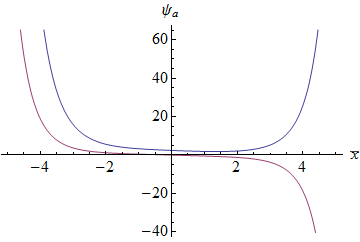
\includegraphics[scale=0.6]{images/magnetic-psi-a}}
		\caption{$\psi_{a}$}
		\label{}
	\end{subfigure}
	\hspace{1.2cm}
	\begin{subfigure}{0.45\textwidth}
		\centerline{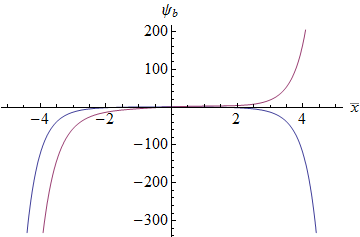
\includegraphics[scale=0.6]{images/magnetic-psi-b}}
		\caption{$\psi_{b}$}
		\label{Magenetic Field wave-functions}
	\end{subfigure}
	\caption{Example plots of wave-function against spacial direction from Equation (\ref{introduction-mag-a}) and Equation (\ref{introduction-mag-b}). Here the wave-functions are shown where the blue curves are the real component and the red curves are the imaginary component. The $\psi_{a}$ component of the graphene wave-function is shown in (a) and the $\psi_{b}$ component is shown in (b).}
	\label{magnetic-psi-a}
\end{figure}
%%%%%
%%%%%
%%%%%
%%%%%
%%%%%
		\section{Density of States}
		\label{Introduction - Density of States}
			The density of states calculation will show the number of available energy states for charge carriers at each energy. Using the linear spectrum of graphene, this calculation can be adapted for the graphene case. The general form of density of states \cite{b3}:
			\begin{equation}
				\rho\left(E\right)=\sum_{k}\delta\left(E-E_{k}\right)
			\end{equation}
			Converting sum notation to integration in two dimensions, the density of states becomes:
			\begin{equation}
				\rho\left(E\right)=\frac{L_{x}L_{y}}{4\pi^{2}}2\int_{k}\int_{\theta}\delta\left(E-E_{k}\right)kdkd\theta
			\end{equation}
			where $L_{x,y}$ is the size of the graphene sheet in the respective direction with 2 spin degeneracy. From the linear spectrum of graphene the relations:
			\begin{align}
				E_{k}=\hbar v_{f}k
				\hspace{1cm}
				dE_{k}=\hbar v_{f}dk
				\hspace{1cm}
				kdk=\frac{E_{k}}{\hbar^{2}v_{f}^{2}}dE_{k}
			\end{align}
			can be made and the density of states becomes:
			\begin{equation}
				\rho\left(E\right)=\frac{L_{x}L_{y}}{2\pi^{2}}\int_{-\infty}^{\infty}\delta\left(E-E_{k}\right)2\pi \frac{E_{k}}{\hbar^{2}v_{f}^{2}}dE_{k}
			\end{equation}
			Using the Dirac delta function rule and 2 valley degeneracy for electrons and holes, the graphene density of states for a linear spectrum becomes \cite{b3}:
			\begin{equation}
				\rho\left(E\right)=\frac{2L_{x}L_{y}}{\pi\hbar^{2}v_{f}^{2}}|E|
				\label{introduction-dos}
			\end{equation}
			If instead of the linear energy spectrum, the graphene spectrum with an energy gap may be used the following adaptations:
			\begin{align}
				E_{k}=\sqrt{\hbar^{2} v_{f}^{2}\left(k_{x}^{2}+k_{y}^{2}\right)+m^{2}}
				\hspace{1cm}
				k=\frac{\sqrt{E_{k}^{2}-m^{2}}}{\hbar v_{f}}
				\hspace{1cm}
				kdk=\frac{E_{k}}{\hbar^{2}v_{f}^{2}}dE_{k}
			\end{align}
			Resulting in the same equation for the linear density of states in graphene.
%%%%%
%%%%%
%%%%%
		\section{Landauer Formalism}
		\label{Introduction - Landauer Formalism}
			It will be useful to determine the current through a graphene nano-device. For a single channel system at non-zero temperatures the current  through the system shown in Figure \ref{introduction-current} can be found \cite{b6}.
			\begin{figure}[h]
				\centerline{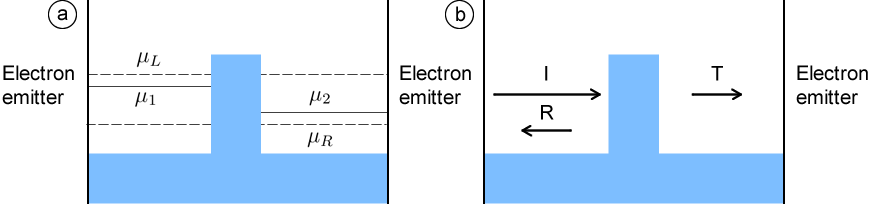
\includegraphics[scale=0.5]{images/current}}
				\caption{(a) Diagram showing quasi-Fermi-energies and chemical potentials of the perfectly conducting wires. Here the left emitter injects electrons up to the quasi-Fermi-energy $\mu_{L}$ and the right emitter injects electrons up the the quasi-Fermi-energy $\mu_{R}$. $\mu_{1}$ and $\mu_{2}$ are the chemical potentials of the perfectly conducting wires to the left and right of the scattering device. (b) A scattering device between two electron emitters. Charge carriers from the left emitter are scattered with a probability $R$ of being reflected and probability $T$ of transmitting through the scattering device.}
				\label{introduction-current}
			\end{figure}
			 The system in Figure \ref{introduction-current} consists of two incoherent electron reservoirs, which emit charge carriers up to the quasi-Fermi-energy $\mu_{L,R}$, where the subscript $L$ and $R$ represent the reservoir at each side of the system. These reservoirs are then connected to a scattering device via perfect and identical one dimensional conductors. These conductors have chemical potentials $\mu_{1}$ and $\mu_{2}$. The current from the left reservoir to the right is then:
			\begin{equation}
				I=ev\frac{dn}{dE}\left(\mu_{L}-\mu_{R}\right)
				\label{current-dos}
			\end{equation}
			The current that is transmitted through the sample is:
			\begin{equation}
				I=\frac{e}{\pi\hbar}T\left(\mu_{L}-\mu_{R}\right)
				\label{current-transmit}
			\end{equation}
			Where the one dimensional density of states $dn/dE=1/\hbar\pi v$. The total number of states in each conducting wire is given by the density of states and the energy range available; $2\left(dn/dE\right)\left(\mu_{L}-\mu_{R}\right)$. On the right side the number of occupied states is therefore $T\left(dn/dE\right)\left(\mu_{L}-\mu_{2}\right)$ and the unoccupied states is then $\left(2-T\right)\left(dn/dE\right)\left(\mu_{2}-\mu_{R}\right)$. The chemical potential of the right wire can then be determined by:
			\begin{equation}
				T\left(dn/dE\right)\left(\mu_{L}-\mu_{2}\right)=\left(2-T\right)\left(dn/dE\right)\left(\mu_{2}-\mu_{R}\right)
				\label{mu-a}
			\end{equation}
			The left wire contains the incident electrons as well as any reflected electrons. The occupied states is then $\left(1+R\right)\left(dn/dE\right)\left(\mu_{L}-\mu_{1}\right)$ and the unoccupied states $\left(2-\left(1+R\right)\right)$ $\left(dn/dE\right)\left(\mu_{1}-\mu_{R}\right)$. An expression for $\mu_{1}$ can then be found:
			\begin{equation}
				\left(1+R\right)\left(dn/dE\right)\left(\mu_{L}-\mu_{1}\right)=\left(2-\left(1+R\right)\right)\left(dn/dE\right)\left(\mu_{1}-\mu_{R}\right)
				\label{mu-b}
			\end{equation}
			The difference in the bottoms of the conduction bands can then be represented by the potential difference:
			\begin{equation}
				eV=\mu_{1}-\mu_{2}
			\end{equation}
			With Equation (\ref{mu-a}) and Equation (\ref{mu-b}) this potential can be represented by $eV=R\left(\mu_{L}-\mu_{R}\right)$. Then with the definition of conductance, this potential difference and Equation (\ref{current-transmit}) the conductance can be expressed as:
			\begin{equation}
				G=\frac{I}{V}=\frac{e^{2}}{\pi\hbar}\frac{T}{R}
				\label{GTR}
			\end{equation}
			At non-zero temperatures the reservoirs do not fully fill the states up to the quasi-Fermi-energies, instead they are filled according to the Fermi-Dirac distributions:
			\begin{equation}
				f\left(E-\mu_{L,R}\right)=\frac{1}{e^{\frac{E-\mu_{L,R}}{k_{b}t}}+1}
			\end{equation}
			where $k_{b}$ is the Boltzmann constant and $t$ is the temperature. With these distributions the quasi-Fermi-energies can be replaced. Then by integrating with respect to energy the current in Equation (\ref{current-transmit}) becomes:
			\begin{equation}
				I=\frac{e}{\pi\hbar}\int T\left[f\left(E-\mu_{L}\right)-f\left(E-\mu_{R}\right)\right] dE
				\label{current-temp}
			\end{equation}
			To find the conductance at non-zero temperatures the chemical potentials in Equation (\ref{mu-a}) and Equation (\ref{mu-b}) must be multiplied by the Fermi distributions and integrated.
			\begin{equation}
				\mu_{1}=\frac{\int\left(\frac{-df}{dE}\frac{dn}{dE}R\left(E\right)\left(\mu_{L}-\mu_{R}\right)+\mu_{L}\right)dE}{\int\frac{-df}{dE}\frac{dn}{dE}dE}
				\hspace{1cm}
				\mu_{2}=\frac{\int\left(\frac{-df}{dE}\frac{dn}{dE}T\left(E\right)\left(\mu_{L}-\mu_{R}\right)+\mu_{R}\right)dE}{\int\frac{-df}{dE}\frac{dn}{dE}dE}
			\end{equation}
 			Where the definition:
			\begin{equation}
				\frac{-df}{dE}=\left[f\left(E-\mu_{L}\right)-f\left(E-\mu_{R}\right)\right]/\left(\mu_{L}-\mu_{R}\right)
			\end{equation}
			will be used. Assuming the velocity has a negligible dependence on energy, the voltage at finite temperature is now:
			\begin{equation}
				eV=\frac{\int \frac{-df}{dE}R\left(E\right) \left(dn/dE\right)dE}{\int \frac{-df}{dE}\left(dn/dE\right)dE}\left(\mu_{L}-\mu_{R}\right)
				\label{voltage-temp}
			\end{equation}
			With Equation (\ref{current-temp}) and Equation (\ref{voltage-temp}) the conductance at non-zero temperatures is:
			\begin{equation}
				G=\frac{e^{2}}{\pi\hbar}\int T\left(E\right)\frac{-df}{dE} dE \frac{\int \frac{-df}{dE}\left(dn/dE\right)dE}{\int \frac{-df}{dE}R\left(E\right) \left(dn/dE\right)dE}
				\label{conductance-temperature}
			\end{equation}
			At zero temperature and with small voltages across the source-drain $\frac{-df}{dE}$ becomes $\delta \left(E-E_{f}\right)$, the integrals are removed by the identity $\int f(x)\delta(x) dx=f(0)$ and Equation (\ref{conductance-temperature}) reduces to Equation (\ref{GTR}). In the case of $R=0$ this result produces infinite conductance. However, \cite{b7} shows that for any length of perfect conductor an electric field can be absorbed and the condition of $R\approx 1$ can be used. For a system with a region of perfect transmission the conductance is given to be:
			\begin{equation}
				G=\frac{e^{2}}{\pi\hbar}T\left(\mu_{L}-\mu_{R}\right)
			\end{equation}
			Therefore the result at non-zero temperatures, with a region of perfect transmission becomes:
			\begin{equation}
				G=\frac{e^{2}}{\pi\hbar}\int T\left[f\left(E-\mu_{L}\right)-f\left(E-\mu_{R}\right)\right]dE
			\end{equation}
%%%%%
%%%%%
%%%%%
		\section{Landauer Formalism in Graphene}
		\label{Introduction - Landauer Formalism in Graphene}
			In this section the Landauer formalism is derived for a graphene scattering device. For a single channel system at non-zero temperatures the current through the system shown in Figure \ref{introduction-current} can be found \cite{b6}.
			 The system in Figure \ref{introduction-current} consists of 2 incoherent electron reservoirs, which emit charge carriers up to the quasi-Fermi-energy $\mu_{L,R}$, where the subscript $L$ and $R$ represent the reservoir at left or right side of the system respectivly. These reservoirs are then connected to a scattering device via perfect and identical one dimensional conductors. These conductors have chemical potentials $\mu_{1}$ and $\mu_{2}$. The current from the left reservoir to the right is then:
			\begin{equation}
				I=ev_{f}\frac{dn}{dE}\left(\mu_{L}-\mu_{R}\right)
				\label{current-dos}
			\end{equation}
			Where $e$ is the electron charge, $v_{f}$ is the Fermi velocity and $dn/dE$ is the density of states. The current that is transmitted through the sample is then:
			\begin{equation}
				I=ev_{f}\frac{dn}{dE}T\left(\mu_{L}-\mu_{R}\right)
				\label{current-transmit-graphene}
			\end{equation}
			Where $T$ is the transmission probability through the scattering device. In \cite{b1} the density of states for a single unit cell of graphene at a Dirac point is given by:
			\begin{equation}
				\frac{dn}{dE}=\frac{2A_{c}}{\pi}\frac{|E|}{\hbar^{2}v_{f}^{2}}
				\hspace{1cm}
				A_{c}=\frac{3\sqrt{3}a^{2}}{2}
			\end{equation}
			The definition $L_{x}L_{y}/A_{c}$ is the number of unit cells in the sample, where  $L_{x}, L_{y}$ is the size of the sample in the respective dimension and $A_{c}$ is the area of the graphene unit cell. As only the $x$ direction current will be considered here, the current in the $x$ direction will be the same in each cell, therefore only the number of graphene unit cells in the $y$ direction will affect the $x$ directional current. This way the quantity $L_{x}$ can be set to one and removed from the calculation. The current through the graphene sample from Equation (\ref{current-transmit-graphene}) in the $x$ direction becomes:
			\begin{equation}
				I_{x}=e\frac{2L_{y}}{\pi \hbar^{2}v_{f}}T\left(E,\theta\right)\left(\mu_{L}-\mu_{R}\right)|E|\cos(\theta)
			\end{equation}
			The energy $\left(E\right)$ and incident angle $\left(\theta\right)$ dependence for $T$ has been included here to allow for the graphene transmission probability. At non-zero temperatures the states are instead filled according to the corresponding Fermi-Dirac distribution.
			\begin{equation}
				f\left(E-\mu_{L,R}\right)=\frac{1}{e^{\frac{E-\mu_{L,R}}{k_{b}t}}+1}
			\end{equation}
			where $k_{b}$ is the Boltzmann constant and $t$ is the temperature. The current must then be integrated over all energies and values of theta to account for all states in the Fermi-Dirac distributions.
			\begin{equation}
				I_{x}=I_{0}\int^{\infty}_{-\infty}\int^{\pi/2}_{-\pi/2}T\left(E,\theta\right)\left[f\left(E-\mu_{L}\right)-f\left(E-\mu_{R}\right)\right]|E|\cos(\theta)dEd\theta
				\label{introduction-i-graphene}
			\end{equation}
			Here, the group of constants $I_{0}=e\frac{2L_{y}}{\pi\hbar^{2}v_{f}}$ has been introduced. At this stage the current shows a similar form to that in \cite{b9, b10}, with the exception that the graphene density of states causes an additional $|E|$ term and the graphene transmission probability introduces a theta dependence. This result for current can then be used with the definition of conductance $G=I/V$ to find the conductance at a finite temperature for graphene. The potential difference $V$ is determined by the number of charges on the left and right of the scattering device. This can be found by considering the chemical potentials of the perfectly conducing wires. The chemical potentials $\mu_{1,2}$ must be between the quasi-Fermi-energies of the electron emitters $\mu_{L,R}$. The positioning of these chemical potentials requires that the number of occupied states (electrons) above $\mu_{1}$ is equal to the number of unoccupied states (holes) below $\mu_{1}$, and likewise for states above and below $\mu_{2}$. As all states below $\mu_{R}$ must be filled, only the energy range between $\mu_{L}$ and $\mu_{R}$ needs to be considered. Allowing for positive and negative velocities the number of states between this range is $2\left(dn/dE\right)\left(\mu_{L}-\mu_{R}\right)$. To the right of the scattering device the number of occupied states is the total number of states available in the wire multiplied by the transmission probability; $T\left(dn/dE\right)\left(\mu_{L}-\mu_{2}\right)$. The number of unoccupied states must therefore be the total number of states available in the wire minus the filled states $\left(2-T\right)\left(dn/dE\right)\left(\mu_{2}-\mu_{R}\right)$. As the number of occupied states is equal to the number of unoccupied states we can write:
			\begin{equation}
				T\left(dn/dE\right)\left(\mu_{L}-\mu_{2}\right)=\left(2-T\right)\left(dn/dE\right)\left(\mu_{2}-\mu_{R}\right)
				\label{mu-2}
			\end{equation}
			On the left of the scattering device the number of occupied states includes those filled by incident and reflected charge carriers $\left(1+R\right)\left(dn/dE\right)\left(\mu_{L}-\mu_{1}\right)$. The number of unoccupied states is then $\left(2-\left(1+R\right)\right)\left(dn/dE\right)\left(\mu_{1}-\mu_{R}\right)$. The number of occupied and unoccupied states must be equal, therefore:
			\begin{equation}
				\left(1+R\right)\left(dn/dE\right)\left(\mu_{L}-\mu_{1}\right)=\left(2-\left(1+R\right)\right)\left(dn/dE\right)\left(\mu_{1}-\mu_{R}\right)
				\label{mu-1}
			\end{equation}
			The potential difference between the two wires caused by the scattering device is then:
			\begin{equation}
				eV=\mu_{1}-\mu_{2}
			\end{equation}
			Using Equation (\ref{mu-2}) and Equation (\ref{mu-1}) the potential difference across the sample is then:
			\begin{equation}
				eV=R\left(\mu_{L}-\mu_{R}\right)
			\end{equation}
			However, at non-zero temperatures the electron emitters fill the states according to the Fermi-Dirac distibutions. To determine the potential difference at non-zero temperatures Equation (\ref{mu-2}) and Equation (\ref{mu-1}) can be multiplied by the available energy range according to the Fermi-Dirac distributions. Here we will define:
			\begin{equation}
				\frac{-df}{dE}=\left[f\left(E-\mu_{L}\right)-f\left(E-\mu_{R}\right)\right]/\left(\mu_{L}-\mu_{R}\right)
			\end{equation}
			and integrate with respect to energy. This produces the potential difference at non-zero temperatures:
			\begin{equation}
				eV=\frac{\int R\left(E,\theta\right) \frac{-df}{dE} \frac{dn}{dE}dE}{\int\frac{-df}{dE} \frac{dn}{dE}dE}\left(\mu_{L}-\mu_{R}\right)
			\end{equation}
			Using this expression for the voltage and the definition of conductance $G=I/V$ the conductance through a scattering device in graphene can be written as:
			\begin{align}
				G_{x}=e^{2}\frac{2L_{y}}{\pi\hbar^{2}v_{f}}\int^{\infty}_{-\infty}\int^{\pi/2}_{-\pi/2}&T\left(E,\theta\right)\left[f\left(E-\mu_{L}\right)-f\left(E-\mu_{R}\right)\right]|E|\cos(\theta)dEd\theta\\
				&\times\frac{\int\frac{-df}{dE} \frac{dn}{dE}dE}{\int R\left(E,\theta\right) \frac{-df}{dE} \frac{dn}{dE}dEd\theta}\frac{1}{\left(\mu_{L}-\mu_{R}\right)}
			\end{align}
			However, the transmission probability in graphene will become one under resonance conditions, Klein tunnelling or if $\theta=0$. This will cause the reflection probability $R$ to become zero and the voltage to become zero. To allow for this we can restrict the calculation to a system with perfect transmission. As any electric field can be absorbed by a finite region of perfect conductor \cite{b7}, the reflection probability over the entire system will become one. This effect may also be caused by introducing many scattering devices \cite{b6} such as measurement probes. By restricting the calculation to perfect conductors with many scattering devices, $R \approx 1$ and the one dimensional conductance for graphene systems will reduce to:
			\begin{equation}
				G_{x}=e^{2}\frac{2L_{y}}{\pi\hbar^{2}v_{f}}\int^{\pi/2}_{-\pi/2} \int^{\infty}_{-\infty} T\left(E, \theta\right)\frac{f\left(E-\mu_{L}\right)-f\left(E-\mu_{R}\right)}{\mu_{L}-\mu_{R}}|E|\cos(\theta) dE d\theta
				\label{introduction-g-t}
			\end{equation}
			At zero temperature and for small voltages, the Fermi distributions become the Dirac delta function centered at the Fermi energy $E_{f}$. With the identity $\int f(x)\delta(x) dx=f(0)$ the zero temperature conductance for small voltages and large systems becomes:
			\begin{equation}
				G_{x}= G_{0}\int^{\frac{\pi}{2}}_{-\frac{\pi}{2}} T\left(E_{f},\theta\right)|E_{f}|\cos(\theta)d\theta
				\label{introduction-g-zero}
			\end{equation}
			Where constants have been grouped so that $G_{0}=e^{2}\frac{2L_{y}}{\pi\hbar^{2}v_{f}}$. This result for conductance includes the Fermi energy, as required from the density of states of graphene and the integration of a Dirac delta function. A similar result for conductance is shown in \cite{b11, b14,b15}, however many published expressions \cite{b4, b13, b16} for conductance do not include this term. The inclusion of the Fermi energy causes the conductance to become linear outside of the step, or barrier region, dramatically changing the result obtained.
%\end{document}